\chapter{SmartZone: Predictive Zoning}
\label{sec:cs3}

Case study 3 extend the zoning system from reacting to changes in occupancy and
temperature, as described in Chapter~\ref{ch:cs2}, to being able to predict
occupancy and temperature. In this case study models that could be used to
predict the occupancy of rooms and the effect of HVAC actuations on room
temperatures are presented. This chapter also presents an approach to using
these models for predictive control of an HVAC system, but to-date have not
implemented or evaluated such a system due to it requiring another one year
study. Instead, we implement the core components of a predictive zoning system:
a predictive thermal model and a predictive occupancy model, and describe how
they could be used to predictively zone an HVAC system.

\section{Predictive Thermal Model}
\label{sec:cs3thermalModel}

In order to implement a predictive zoning controller the effects of opening or
closing air vent registers on room temperatures have to be predicted. Making such
a prediction is complicated by the fact that weather has a larger effect on room
temperatures than the settings of air vent registers, making it hard to isolate
the influence of the HVAC system. A technique for dynamically estimating the
heat load due to weather on room temperatures and subtracting it out in order to
predict the effect of the HVAC system more directly is presented.

\subsection{Introduction}
\label{sec:introduction}

\newcommand{\tab}{\hspace*{2em}}

A predictive zoning controller needs to be able to predict the effect of opening
or closing registers on the room temperatures. Thus, this section describes and
evaluates techniques to learn and predict the effect of opening or closing each
vent register, in a set of {\em R} air vent registers, on the temperature at
each sensor, in a set of {\em T} temperature sensors placed within a house.

The main challenge to modeling the thermal characteristics of a house is
the effect of weather on the indoor temperature. For instance, wind, solar gain,
and outdoor temperature have a greater influence on indoor temperature than any
individual air vent register. It is difficult to build a model that completely
captures the effect of weather on indoor temperatures because outdoor weather
conditions constantly change and rarely repeat. The difficulty of attributing
the influence on weather conditions on indoor temperature makes it difficult to
isolate the effect of the state of any particular air vent register on the
indoor temperature.

This problem is overcome by modeling the indoor temperature in two stages. In
the first stage, the rate of heat gain or loss due exclusively to outdoor
weather conditions is measured. This stage is modeled with data collected when
the HVAC system is off using a linear function of current temperature. Then,
when the HVAC system is turned on, the {\em change} in the rate of heat gained
or lost in a room due to the conditioned air provided by the HVAC system is
measured. This change is expected to be constant throughout the year because the
HVAC system always outputs the same amount of conditioned air. Thus, the HVAC
effects are isolated by learning and subtracting out a dynamic estimate of
weather effects over long periods of time.

This section describes three iterations of a thermal model and analyze its
accuracy in terms of predicting the effect of opening and closing various
combinations of registers with a centralized HVAC system. Ten-fold cross
validation over three weeks of data sampled over three months is used to
demonstrate that even with the simplest model temperatures can be predicted to
within two degrees 30 minutes into the future. A 30 minute time window is
considered because longer time windows are not beneficial when making HVAC
control decision. Even the simplest of the three models presented in this
section is able to provide this level of accuracy allowing temperature
prediction to be incorporated into an HVAC zoning controller easily and without
much computation overhead.

\subsection{Background and Related Work}
\label{sec:thermalBackground}

%% gives a basic idea of how a HVAC system and zoning work.  This is similar to
%% your current section called "system characteristics".  Don't go into too much
%% detail about the zoning system, because that will be published in other
%% venues.

In order to evaluate the energy efficiency of buildings and implement building
energy control strategies, a number of methods have been proposed to model the
thermal performance of building envelopes. Well mixed
models~\cite{haves1998standard, ahmed1996model}, thermal bridge
models~\cite{carpenter2001advances}, mixed convection heat transfer
models~\cite{beausoleil1999modelling}, and CFD models~\cite{peng1996modeling,
ratnam1998advanced} are just a few examples of temperature response models that
were developed for buildings. These techniques rely on modeling the building in
detail using software such as DOE-2~\cite{birdsall1990overview} and
COMIS~\cite{feustel1999comis} which are then used to predict the thermal flow
across zones. This approach is infeasible for a system deployed by a non-expert
homeowner since modeling a house in detail is not easy even for experts.

Mozer et al.~\cite{mozer1997neurothermostat} use an RC model of the Neural
Network House, where their Neurothermostat is evaluated. This model assumes that
the inside, and outside, of the house are at uniform temperatures, the walls
have a thermal resistance, {\em R}, and thermal capacitance, {\em C}, the entire
wall mass is at the inside temperature, and the heat input to the inside is {\em
  Q} when the furnace is running or zero otherwise. Using these assumptions, and
constants for {\em R} and {\em C} determined from the architectural properties
of the house, the thermal model was used to predict the future indoor
temperatures as a function of the outdoor temperature and the furnace
operation. 

\subsection{Problem Definition}
\label{sec:problem}

%% Add a section called "problem definition" that really dives in deeper into
%% why this is a hard problem. you have multiple registers and multiple
%% temperature sensors, and want to answer the question "how much does each
%% register affect the value of each temperature sensors?".  A secondary
%% question you would like to ask is "can we learn this without knowing the
%% weather during the training phase?  And can we learn this without know which
%% registers and temperature sensors are in the same room, i.e. self
%% configuration?"

\begin{figure}
\begin{center}
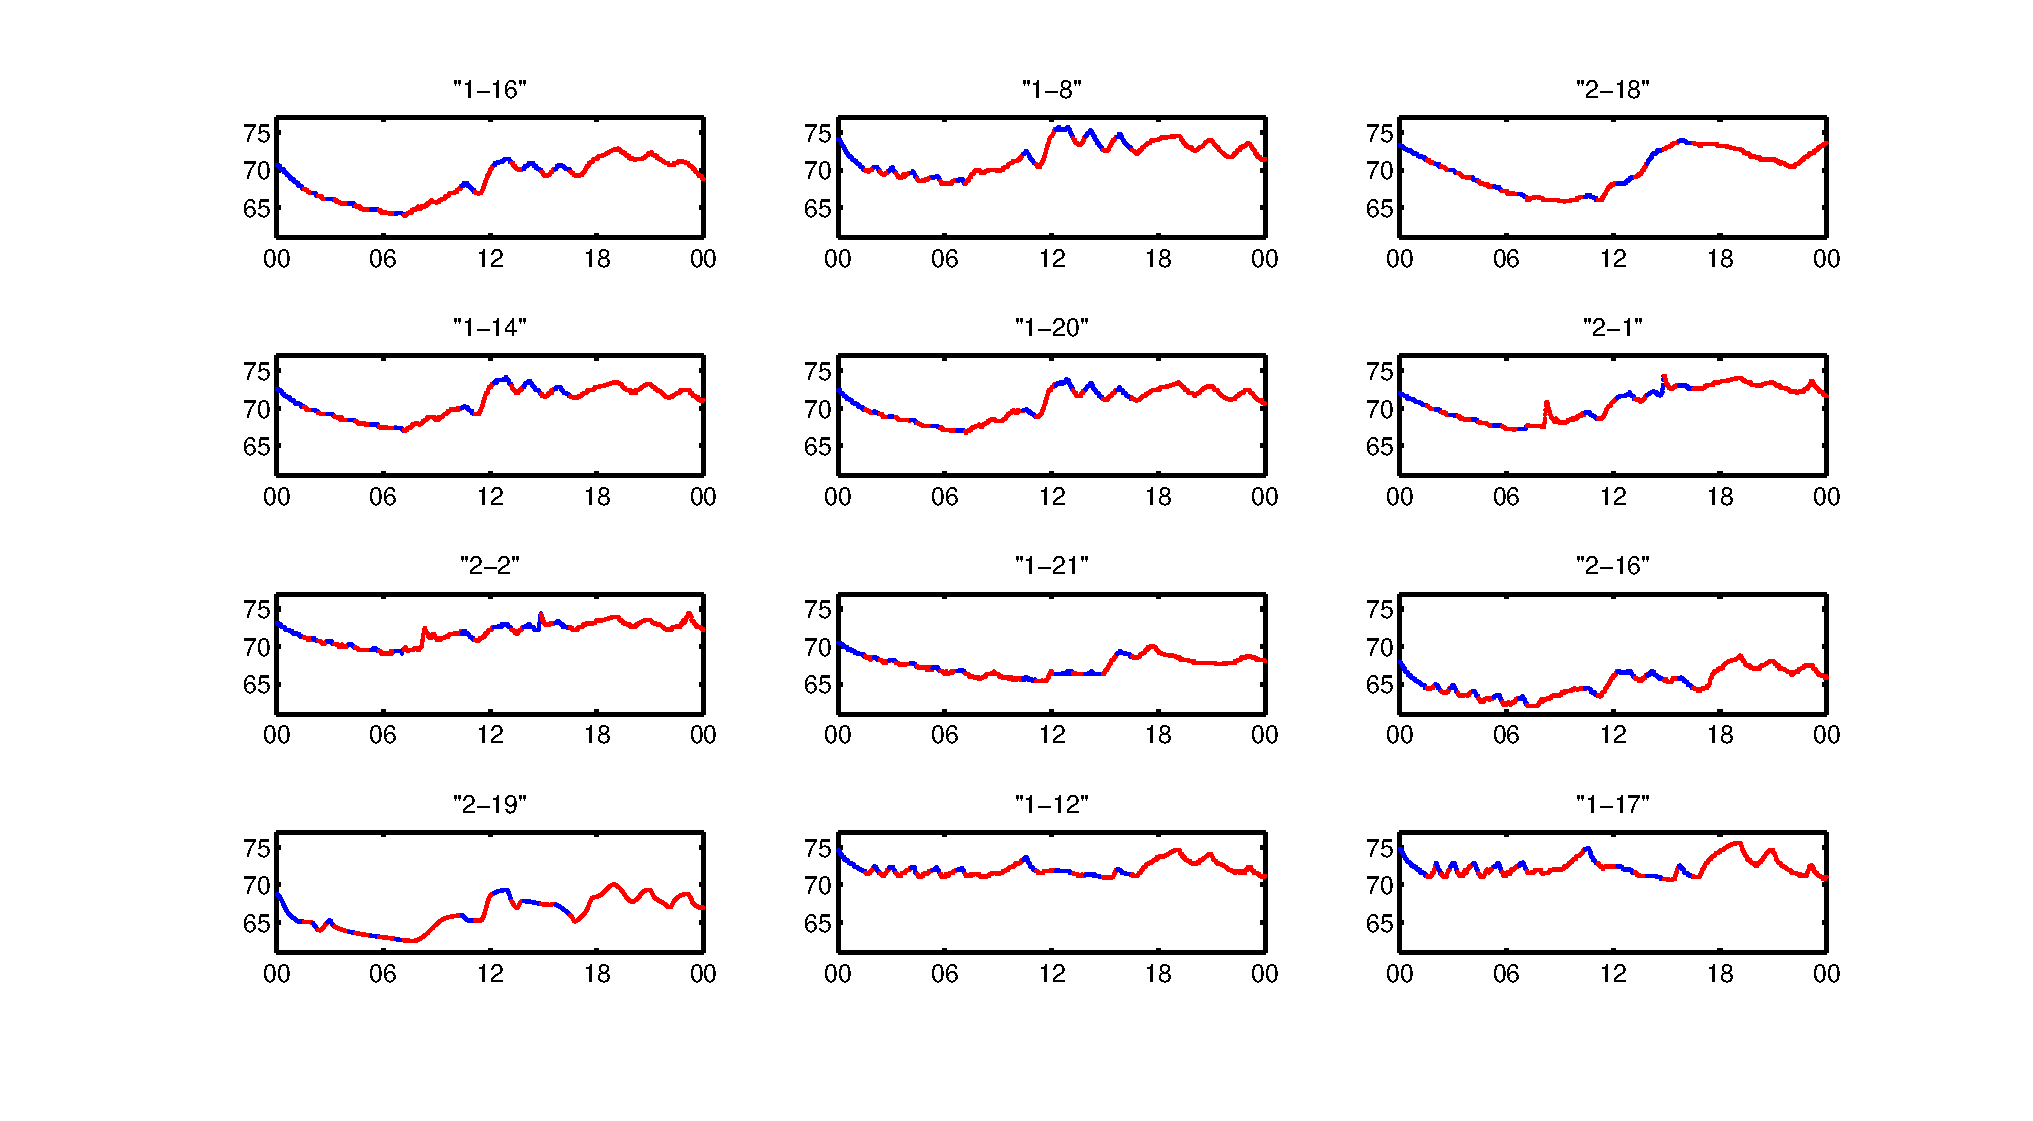
\includegraphics[width=0.8\columnwidth]{fig/1daytemponoff.eps}
\end{center}
\caption[Effect of HVAC system on temperature sensors]{The effect on temperature
sensors, within a 24-hour period, of the HVAC system being on (red) and off
(blue) when heating with all air vent dampers open. The locations of the twelve
sensors are presented in Figure~\ref{fig:cs1Floorplan}}
\label{fig:hvacOnOffAffect}
\end{figure}

The temperature prediction problem is defined by a set of air vent dampers {\em
D} and a set of temperature sensors {\em T} that are dispersed across a house
(Figure~\ref{fig:cs1Floorplan}). The dampers can be opened or closed,
determining if conditioned air is delivered directly into a room. Due to the
lack of thermal isolation between rooms, even if the air vent dampers of a room
are closed, its temperature could still be affected by the HVAC system due to
leakage from neighboring rooms. The temperature sensors monitor the temperatures
at different points throughout the house. Figure~\ref{fig:hvacOnOffAffect} shows
the readings at the twelve temperature sensors in the deployment during a day
with all air vent dampers open. As the figure shows, the HVAC system being off
(blue) causes drops in temperature while the HVAC system being on (red) usually
causes temperature increases. The goal is to learn and predict these effects on
the temperature sensors when different sets of air vent dampers are opened and
closed. In other words, the thermal model is attempting to answer the question
{\em ``What effect does each register being open have on the reading of each
temperature sensor?''}  Being able to make such a prediction allows the
implementation of a finer-grained automated zoning controller that can
dynamically alter zones within a single floor to maintain occupied rooms at a
comfortable temperature while allowing unoccupied rooms to drift. Yet, answering
this question is difficult due to the effect of the weather on the internal
temperature of houses. Wind, solar gain, outdoor temperature, and other weather
conditions have a much greater influence on indoor temperature than the
conditioned air provided by an HVAC system. These weather conditions constantly
change, and rarely repeat, therefore including it as part of a model is
impossible without greatly increasing the complexity of the model. But, ignoring
the effect of weather on internal temperature makes it impossible to isolate the
effect of a particular register on a temperature sensor. Thus, a secondary
question that this section attempts to answer is {\em ``Can the effect of
dampers on temperature sensors be learned without knowing the weather during the
training phase?''} In other words, the model attempts to capture the effect of
the weather on the temperature sensor readings while ignoring the actual weather
conditions, such as the external temperature or the position of the sun.

There have been a number of approaches proposed for learning the thermal
response of buildings in order to control HVAC systems
efficiently~\cite{Henze2004,Deng2010,Oldewurtel2010,Ma2011,Nghiem2011,Aswani2011}. Yet,
these approaches require a large amount of data or sophisticated sensors that
will hinder the goal of developing a cheap and easy to install retrofit to
enable room-level zoning of existing centralized HVAC systems.

\subsection{Experimental Setup}
\label{sec:experimentalSetup}

%% should be similar to your current section called "residential testbed".  it
%% should give an overview of the house floorplan, the temp sensors that are
%% used, and the heating and zoning system that is installed.

The room-level zoning system described has been deployed in a single-story,
8-room, 1,200-square-foot residential building. A model of the home is shown in
Figure~\ref{fig:cs1Floorplan}. The hallway and porch are depicted, but not included
within the analysis because of the inability to actuate temperature within these
regions. The HVAC system setup is overlaid in order to show the position of
vents, ducts, and the central air handler.

% \begin{figure}
% \begin{center}
% 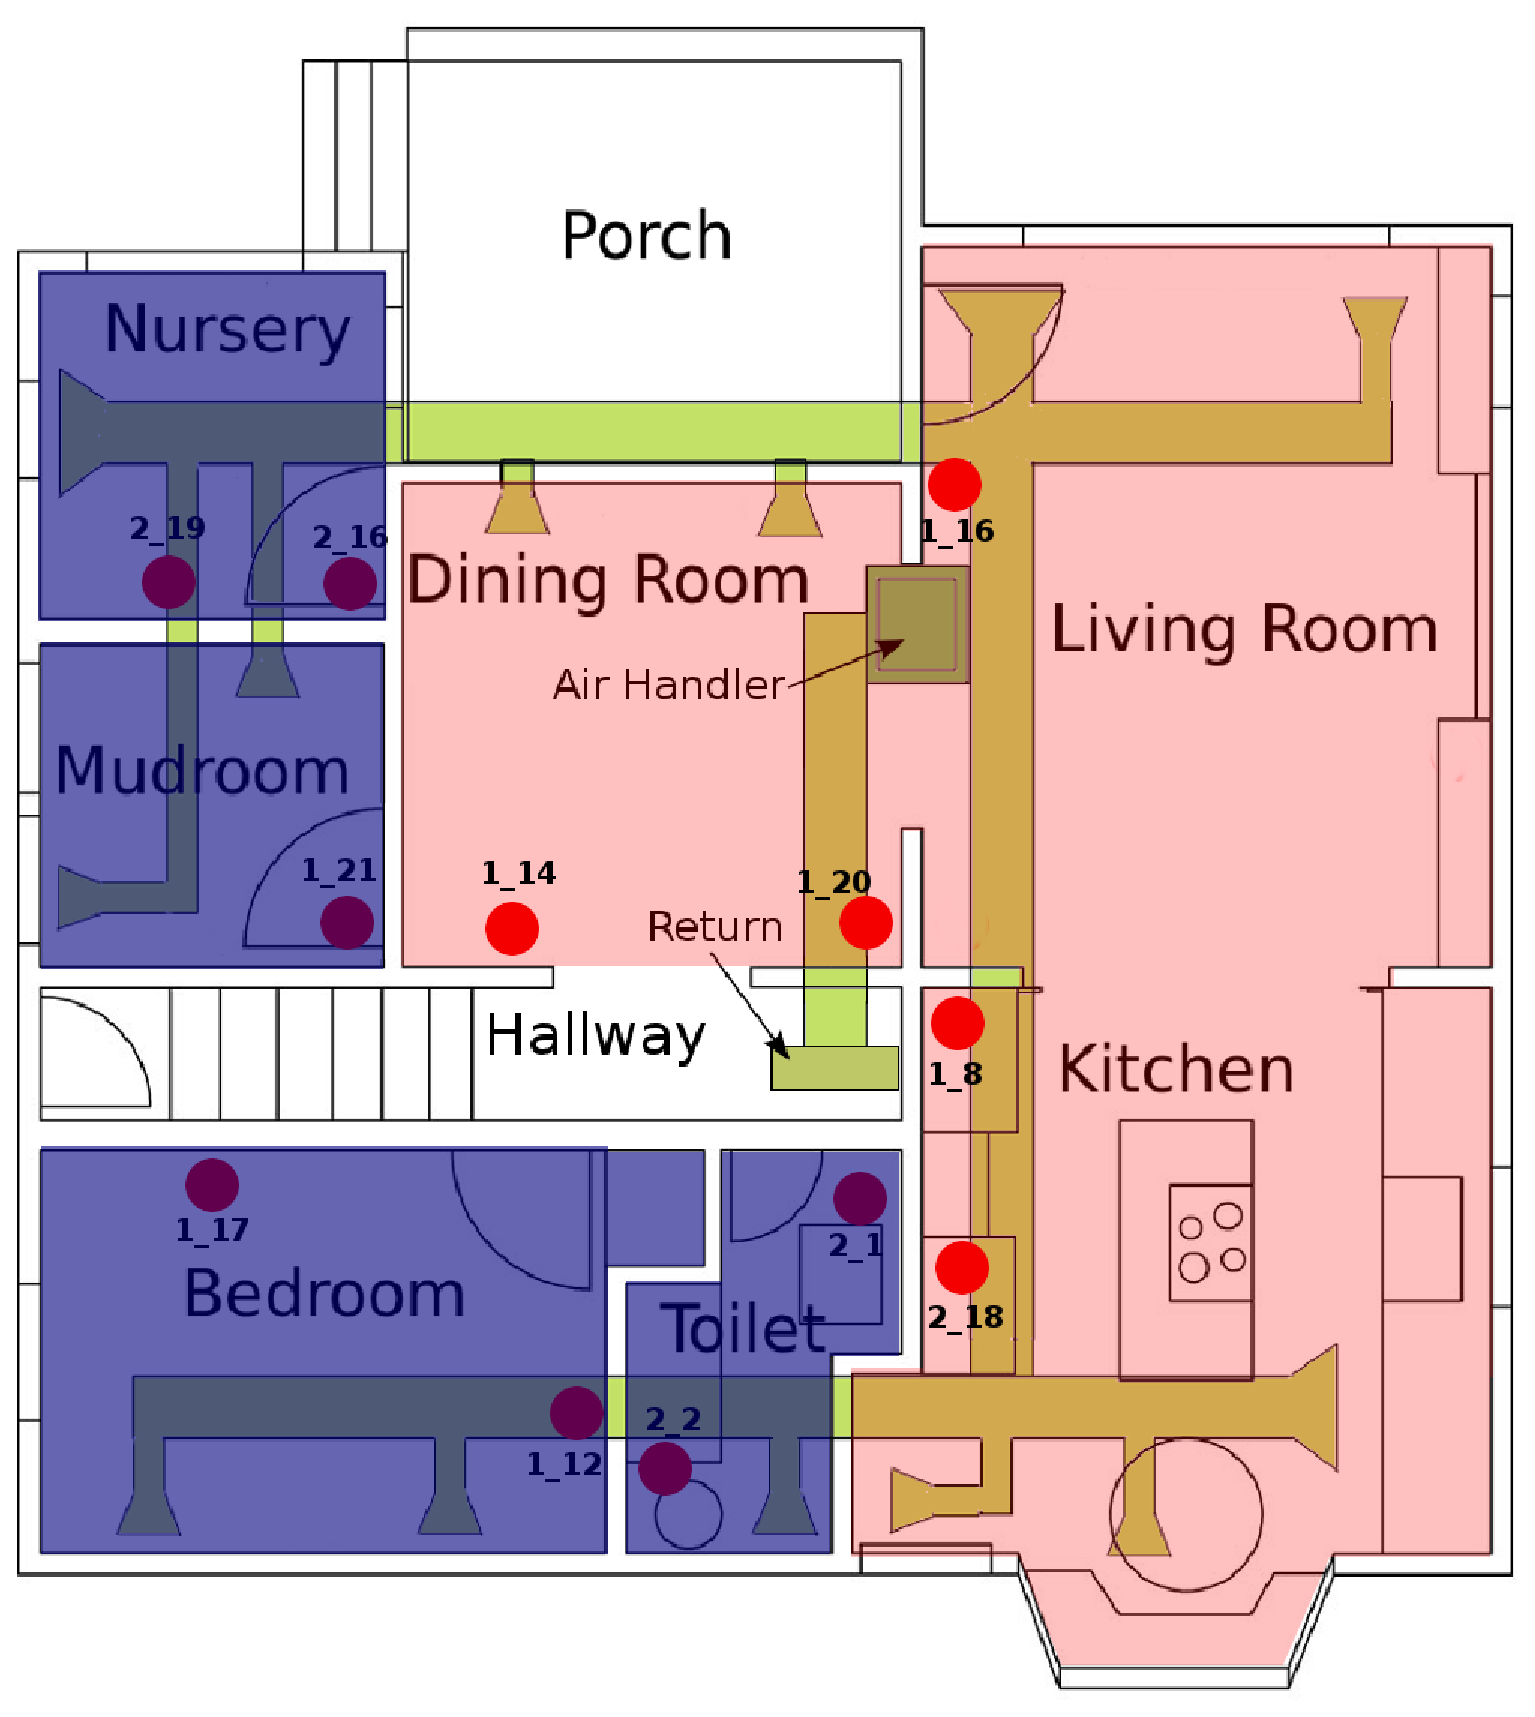
\includegraphics[width=0.6\columnwidth]{fig/floorplan-withTempSensors.eps}
% \end{center}
% \caption[Floorplan showing temperature sensor deployment]{The residential
% testbed used for this study. Red and blue overlays show an example of two
% room-level zones, the green ducts terminate in air vent registers that can be
% opened or closed, and the red circles show the locations of the twelve
% temperature sensors with the sensor IDs indicated.}
% \label{fig:thermalFloorplan}
% \end{figure}

Figure~\ref{fig:cs1Floorplan} shows the deployment from which data for
evaluating the thermal model was collected. Twelve temperature sensor deployed
across the house and air vent registers that are remotely actuatable are used to
collect data over a three month period. Three weeks of the collected data was
used for the analysis presented in this case study.

\subsection{Model of Temperature Dynamics}
\label{sec:model}

%% It should be similar to your section IV.  However, you should have at least
%% three subsections, each of which describes a different version of your model.
%% discuss a simple model first and then discuss more complex models, e.g. model
%% the thermal coupling between adjacent rooms.

%% discuss and compare a few of the models that you've tried.  Perhaps single
%% register/temperature model, a vector of registers, and a vector of
%% registers/temperatures. This may be the only venue where you really get to
%% publish analysis of the models that didn't work as well.

%There are many challenges associated with creating a model for the system
%described. One is that HVAC systems themselves are large and highly
%variable. The parameters are complex, and the model is often non-linear with
%respect to the temperature dynamics. The particular application of this model
%presents another challenge, in that there is a trade-off between the complexity
%of the model and its computability. While we aim to create a robust model of
%the system, it cannot be too complex, or it may ultimately risk the
%effectiveness of using the model within a control scheme.

%These challenges are compounded by the fact that we have created a predictive
%model using experimental data. This is difficult because the raw data is not
%always rich enough to allow for robust model development. Furthermore, the data
%itself presents difficulties from limitations and errors inherent within the
%sensor networks.

The parameters of the model include the position of the damper, temperature,
system status, and time. These values are recorded through a wireless sensor
network deployed in the testbed and stored in a database. The temperature values
are measured in degrees Fahrenheit, and the damper positions take one of two
values: 0 (closed) or 1 (open 100\%). The system status allows the model to see
whether the system is in off, heat/cool 1, or heat/cool 2 mode. An example of
the damper, temperature, and system status for one room is shown in
Figure~\ref{parameters}.

\begin{figure}
\begin{center}
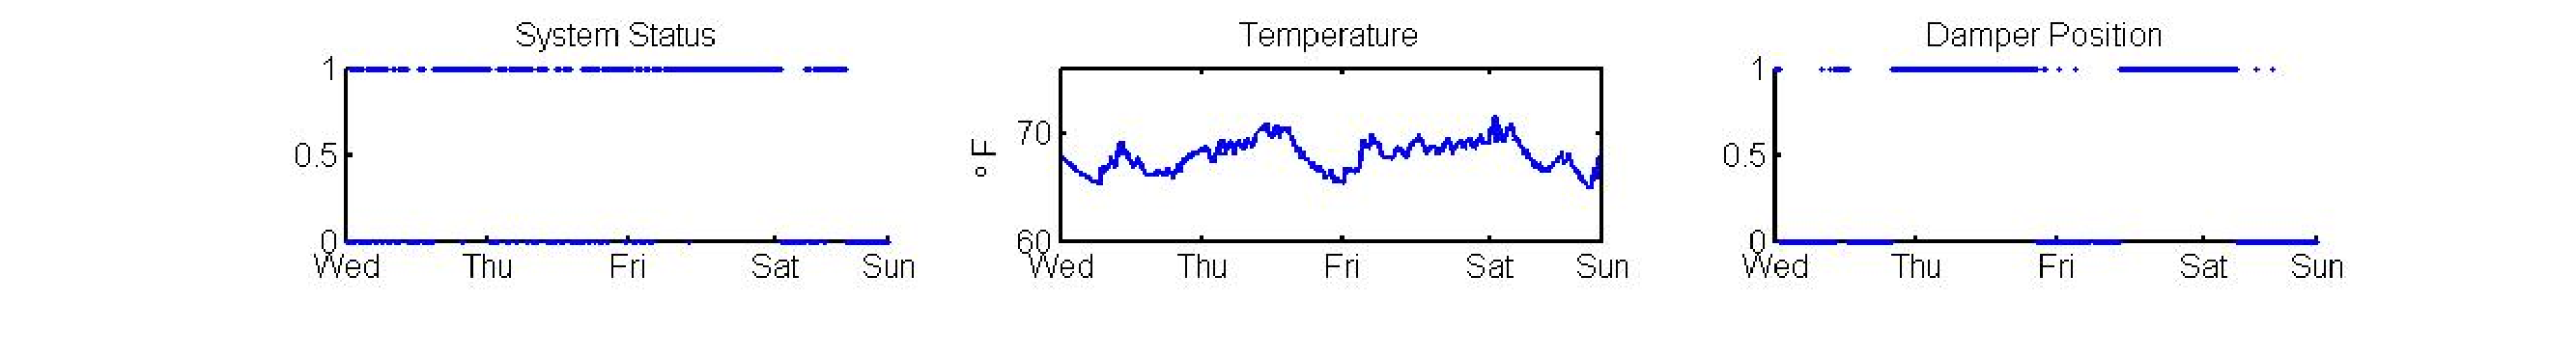
\includegraphics[width=0.8\columnwidth]{fig/parameters.eps}
\end{center}
\caption[Example system parameters collected over one week]{The system status
(on/off), temperature ($^{\circ}$F), and damper position (open/closed) for one
room in the testbed over the period 11/30/2011-12/04/2011.}
\label{parameters}
\end{figure}

In analyzing this system, a number of different models are explored. Three
iterations of the final model are shown in the following sections. Each is a
dynamic, linear model that is developed in two stages. The first stage aims to
estimate the effects of heating/cooling due to external factors such as solar
radiation, wind, and cloud coverage. This effect is calculated when the system
is turned off, and the values are then used to develop the model when the system
turns back on. This two-stage approach allows the compensation for external
factors without having to measure them directly. Furthermore, the results allow
the prediction of temperature dynamics due to the HVAC configuration with
greater accuracy.

\begin{equation}\label{basiceq}dT_k/dt=\alpha T+\beta D\end{equation}

The models discussed follow the same format (Equation~\ref{basiceq}) in which
the temperature of a specific room $T_k$ over time $t$ is a result of external
factors (calculated through $\alpha$), and the current damper configuration,
$D$. The three iterations of this model differ in the way that the external
factor coefficient, $\alpha$, is calculated. These differences are as follows:
1) The first iteration calculates a universal $\alpha$ value by pooling the data
when the system is off. 2) The second iteration calculates a constantly changing
$\alpha$ value when the system is off, and uses this constantly calculated
$\alpha$ value in the model when the system turns on. 3) The third iteration
adds to the model complexity by using universal $\alpha$ values for all
neighbors $T_1, ..., T_n$ of the temperature in room $k$, $T_k$.

\subsubsection{Static $\alpha$}
\label{sec:constantalpha}

The first iteration of the model described is one in which the $\alpha$ values,
which estimate the temperature change due to weather patterns, are constant
throughout the day. In order to calculate these values, the data from times when
the system is off is pooled together and fit one $\alpha$ value across all
timesteps for each of the $n$ rooms. This value is calculated through linear
regression, and assumes that the heat load due to weather remains relatively
constant throughout the day.

\subsubsection{Dynamic $\alpha$}
\label{sec:dynamicalpha}

In the second iteration, the idea that the heat load due to weather conditions
may be changing continuously throughout the day is explored. In order to do
this, a dynamically changing $\alpha$ value is calculated for each off segment,
and include that value in the on segment that directly follows it. This method
aims to compensate for weather by assuming that the heat load due to weather
changes significantly throughout the day, but by very little between one cycle
of the system.

\subsubsection{Adjacency Model}
\label{sec:adjmodel}

The third iteration increases the complexity of the first by including the other
$n$ rooms into the model. This assumes that the current temperature of the room
is affected not only by its own weather conditions, but also by the temperature
dynamics within the other rooms of the building. This model also calculates the
$\alpha$ values universally through linear regression. The form of this room
adjacency model is as follows:

\begin{equation}\label{adjeq}dT_k/dt=\alpha_1T_1+\alpha_2T_2+
  \dots+\alpha_nT_n+\beta D \end{equation}

\subsection{Analysis}
\label{sec:analysis}

%% Add an analysis section with a "training time" analysis.  In other words,
%% re-run the analysis that you have using an increasing number of training days
%% (ranging from, e.g. 5 days to 30 days) to show how quickly each model
%% converges.  You might also have other analysis.

Visually examining the measured and predicted temperatures
(Figure~\ref{fig:predVsMeasured}) highlights a few modeling errors. One is that
the predicted temperatures fail to predict periods of rapidly changing
temperature. However, because the temperatures within this region are acting
within a narrow range, this rapid change is likely to appear as noise to the
system, and is reasonably captured by the predictive model.

\begin{figure}[!htb]
\begin{center}
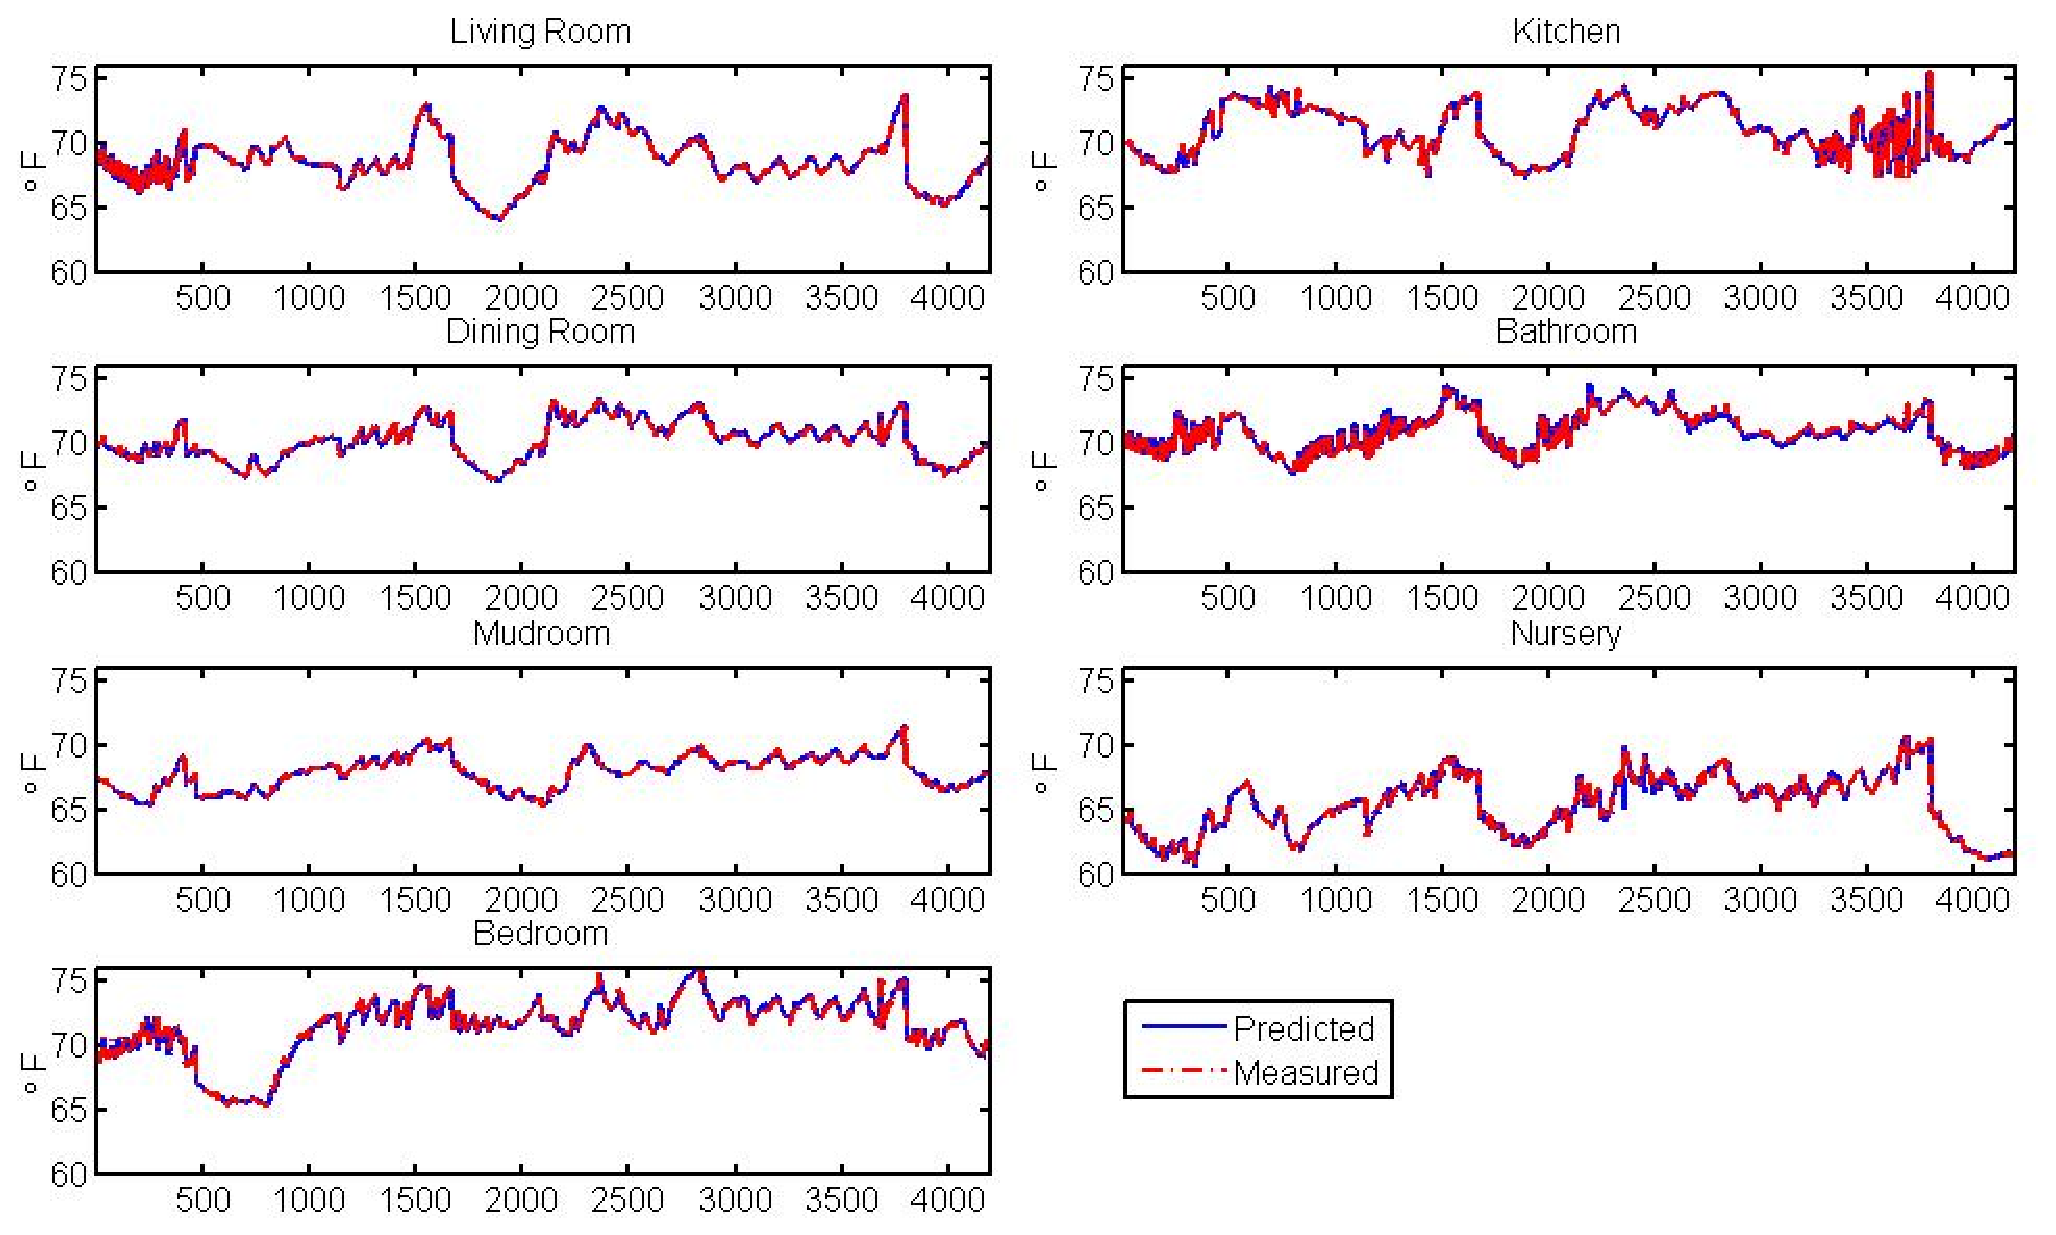
\includegraphics[width=0.8\columnwidth]{fig/predVsMeasured.eps}
\end{center}
\caption[Predicted and measured temperatures]{A plot of the predicted and
measured temperatures when the HVAC system turns on.}
\label{fig:predVsMeasured}
\end{figure}

Another visible error is that the predicted temperatures fail to capture the
temperature magnitude in some cases throughout the week. The largest error is
about 4 degrees Fahrenheit, a value which may be due in part to lost sensor
data. Although this may appear large, it still lies within an interval that
would ensure comfortable temperatures to occupants when creating a control
scheme. Furthermore, the average error is .1064 $^{\circ}$F, which is
quite low and would certainly ensure comfort and precision within the
system. Another indication of a good fit is that the root-mean-square error
(Table~\ref{table:rmsError}) for this prediction is relatively low.

\begin{table}[!htb]
  \caption{Root Mean Square Errors}
  \centering
  \begin{tabular}{| l | c |}
    \hline
    Room & RMS Error ($^{\circ}$F)\\ \hline
    Living Room & 0.2037 \\ \hline
    Kitchen & 0.3248 \\ \hline
    Dining Room & 0.1228 \\ \hline
    Bathroom & 0.3515 \\ \hline
    Mudroom & 0.0847 \\ \hline
    Nursery & 0.1858 \\ \hline
    Bedroom & 0.2160 \\
    \hline
  \end{tabular}
  \label{table:rmsError}
\end{table}

One difficulty in analyzing the effectiveness of this model is the goal of using
it to predict temperatures more than one step in advance.  This involves
calculating predictions at each point that the system is on, up to $t$ minutes
into the future until the system turns off again. This analysis is visualized by
showing the distribution (within two standard deviations) of the model errors
aggregated over each prediction, {\em x} minutes into the future.

\begin{figure}
\begin{center}
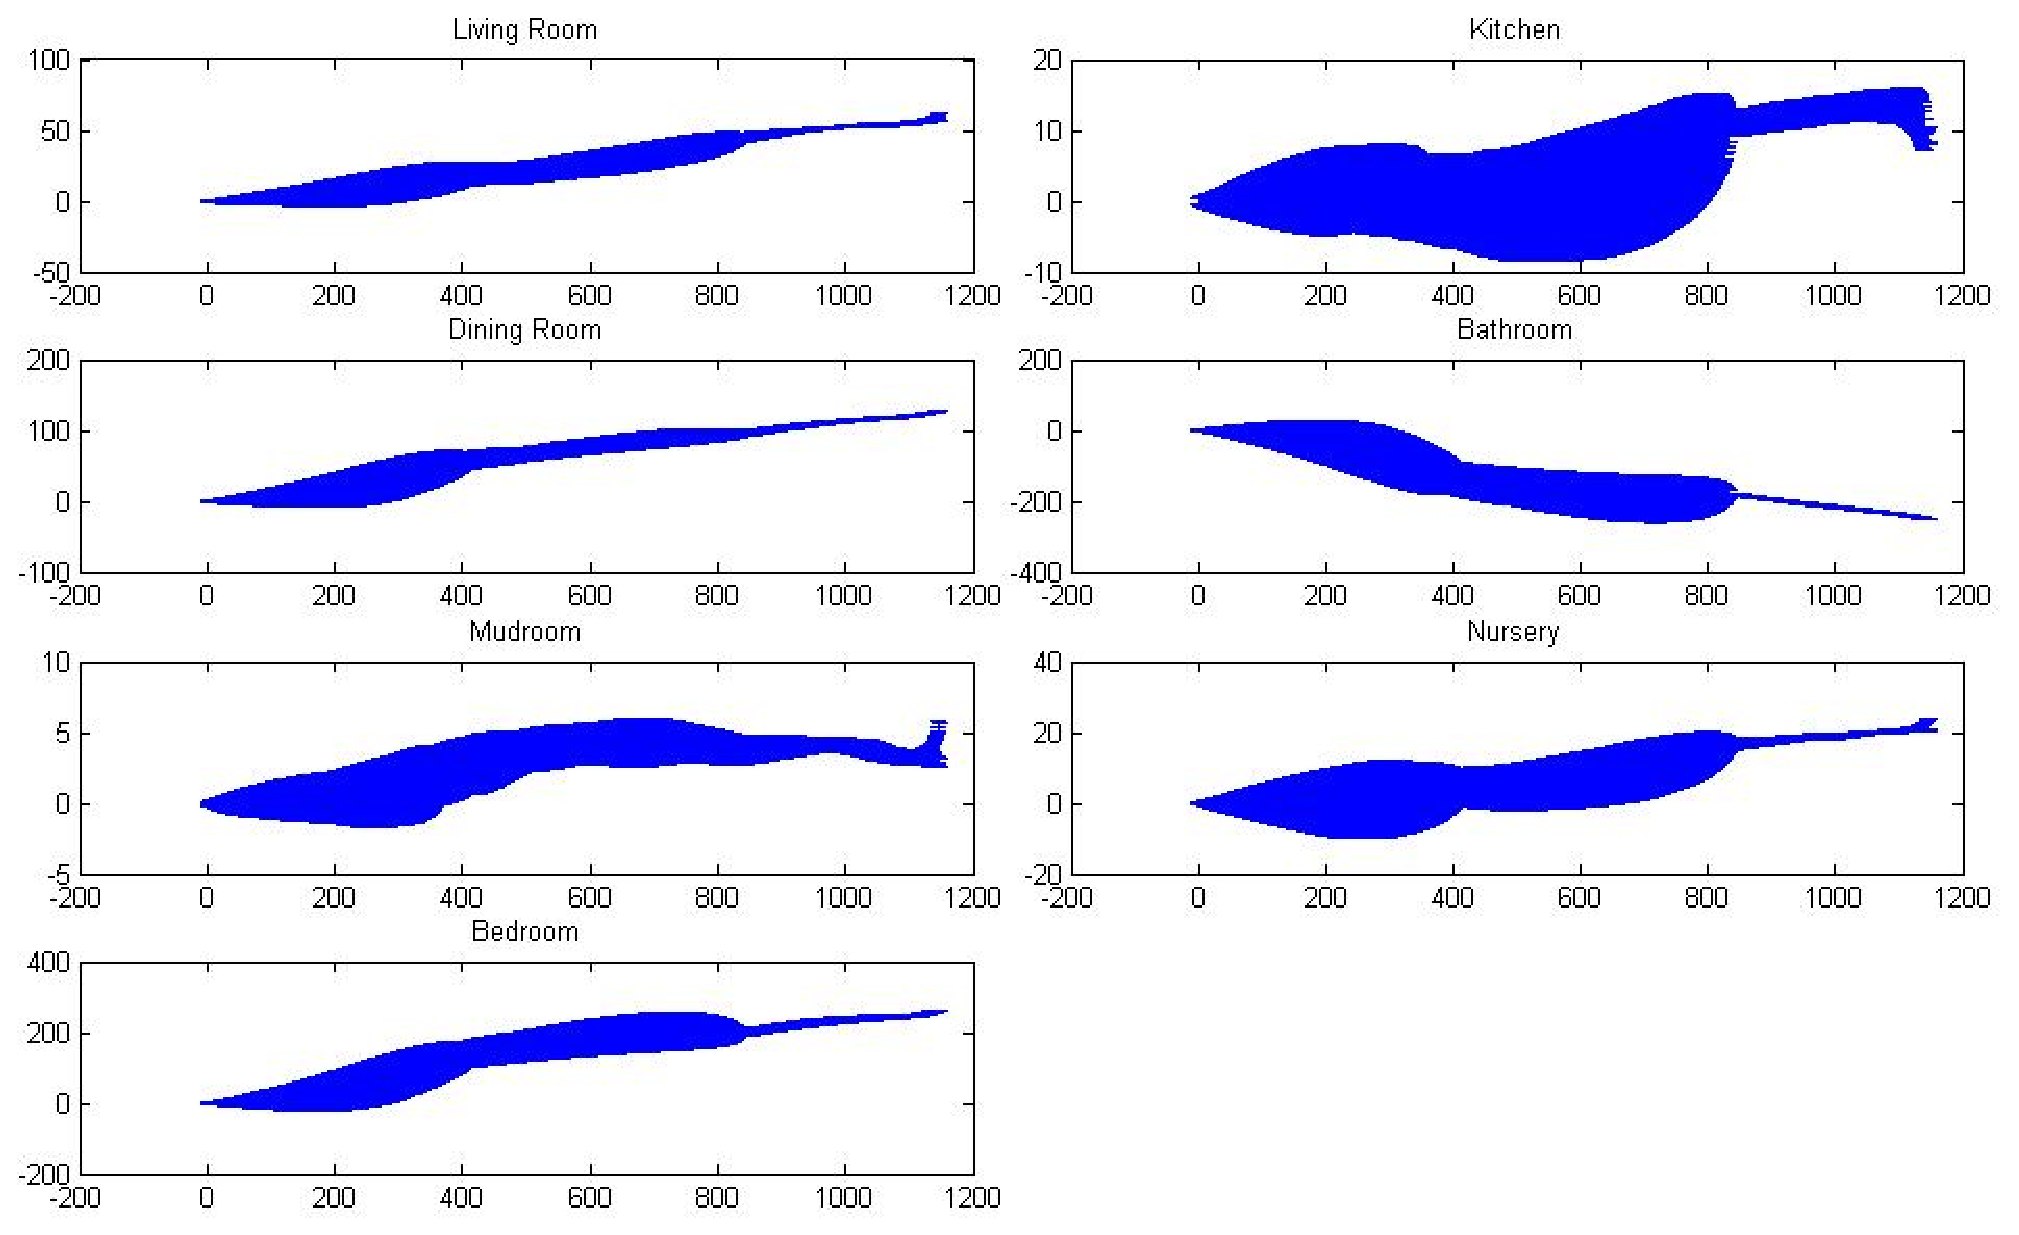
\includegraphics[width=0.8\columnwidth]{fig/errorDist.eps}
\end{center}
\caption[Aggregate plot of error distribution]{Aggregate plot of error
distributions for each prediction, {\em x} minutes into the future.}
\label{fig:errorDist}
\end{figure}

Figure~\ref{fig:errorDist} shows that the error rates are much worse for some
rooms than for others. These rates correspond directly to the $\beta$ values
calculated for these models. That is, the greater the $\beta$ values for a given
room, the worse that it may do in the extreme long-term prediction. This is
because the predicted values grow linearly over time despite nonlinear
temperature dynamics.

However, within a realm of reasonable prediction (less than 30 minutes), the
predictions all do fairly well. As can be expected, the average errors tend to
increase as predictions are made further into the future. The variance of these
errors also increases until a certain point, in which case the errors all become
more uniformly skewed.

\subsection{Results}
\label{sec:thermalResults}

%% analyze and compare results from all of the models.  Give multiple graphs,
%% including example traces and overall error.  It can also include the
%% percentage accuracy graph that we discussed today.  

Three iterations of the model described in section 5 are compared using 21 days
worth of data tested with 10-fold cross validation which involves randomly
dividing the 21 days of data into ten equal sets, training the model using nine
of those sets, and testing with the remaining set. All combinations of nine sets
for training and one set for testing are used. The 21 days selected for model
development and testing have been sampled from 3 months worth of data between
October and December 2011. Using the training data, the $\beta$ values for the
model are developed. These values are then used with the $\alpha$ value scheme
dictated by the model iteration in order to predict temperatures when the system
turns on.

\subsubsection{Prediction}
The predictions assume that temperature grows linearly when the system turns on
as a result of the current damper configuration and the previous weather
patterns estimated through $\alpha$. Though temperature dynamics within a
building are often nonlinear, a reasonable estimate is found by predicting
temperature linearly into the future. This is because the temperature and
airflow of the system operate within a narrow regime, making it reasonable to
approximate change with a linear model. An example of a prediction 30 minutes
into the future is shown in Figure~\ref{fig:expred}. Here, the blue lines
represent the actual temperatures and the red line plots the prediction. The
solid blue line shows the temperature when the system is off, and the red/blue
dashed lines show the predicted/actual temperatures when the system has just
turned on.

\begin{figure}
\begin{center}
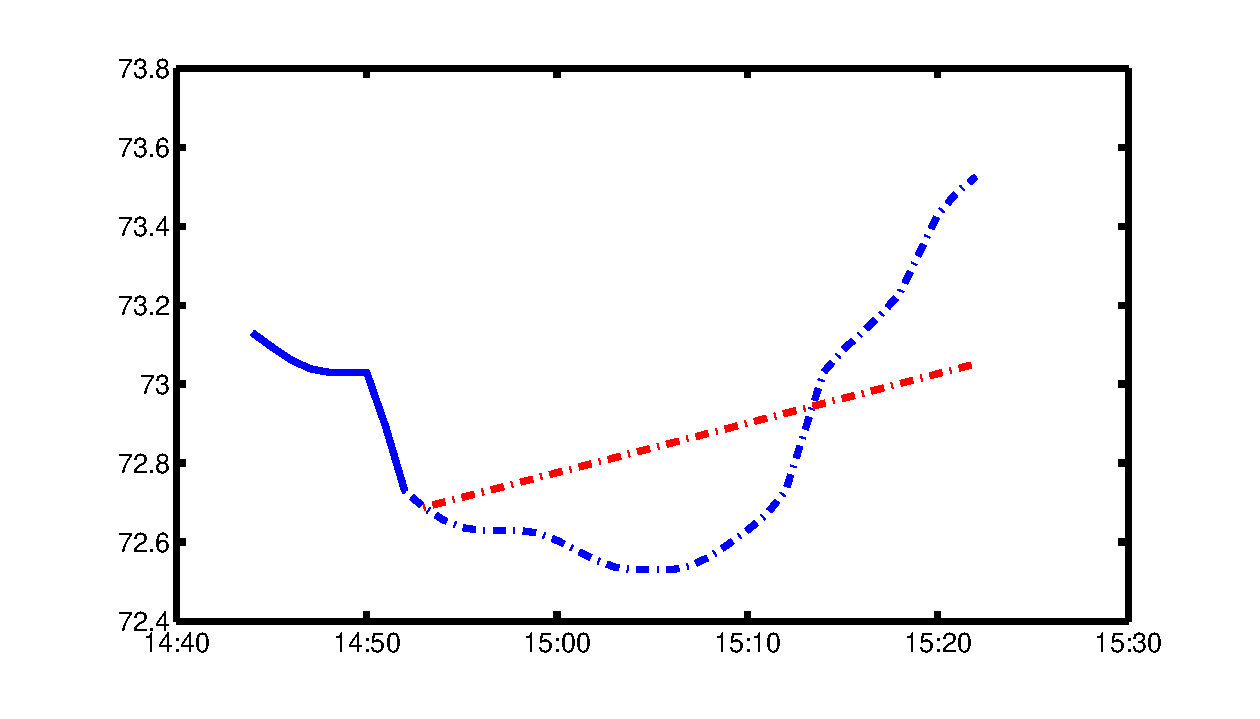
\includegraphics[width=0.6\columnwidth]{fig/ExamplePrediction.eps}
\end{center}
\caption[Example of a temperature prediction]{An example of a prediction made
for temperature up to 30 minutes into the future after the system turns on. The
solid blue line shows the actual temperature when the system is off; the dashed
blue line shows the actual temperature when the system is on; and the dashed red
line shows temperature predicted after the system has just turned on.}
\label{fig:expred}
\end{figure}

\subsubsection{Error Metric}
\label{sec:errormetric}

\begin{figure}[!htb]
\begin{center}
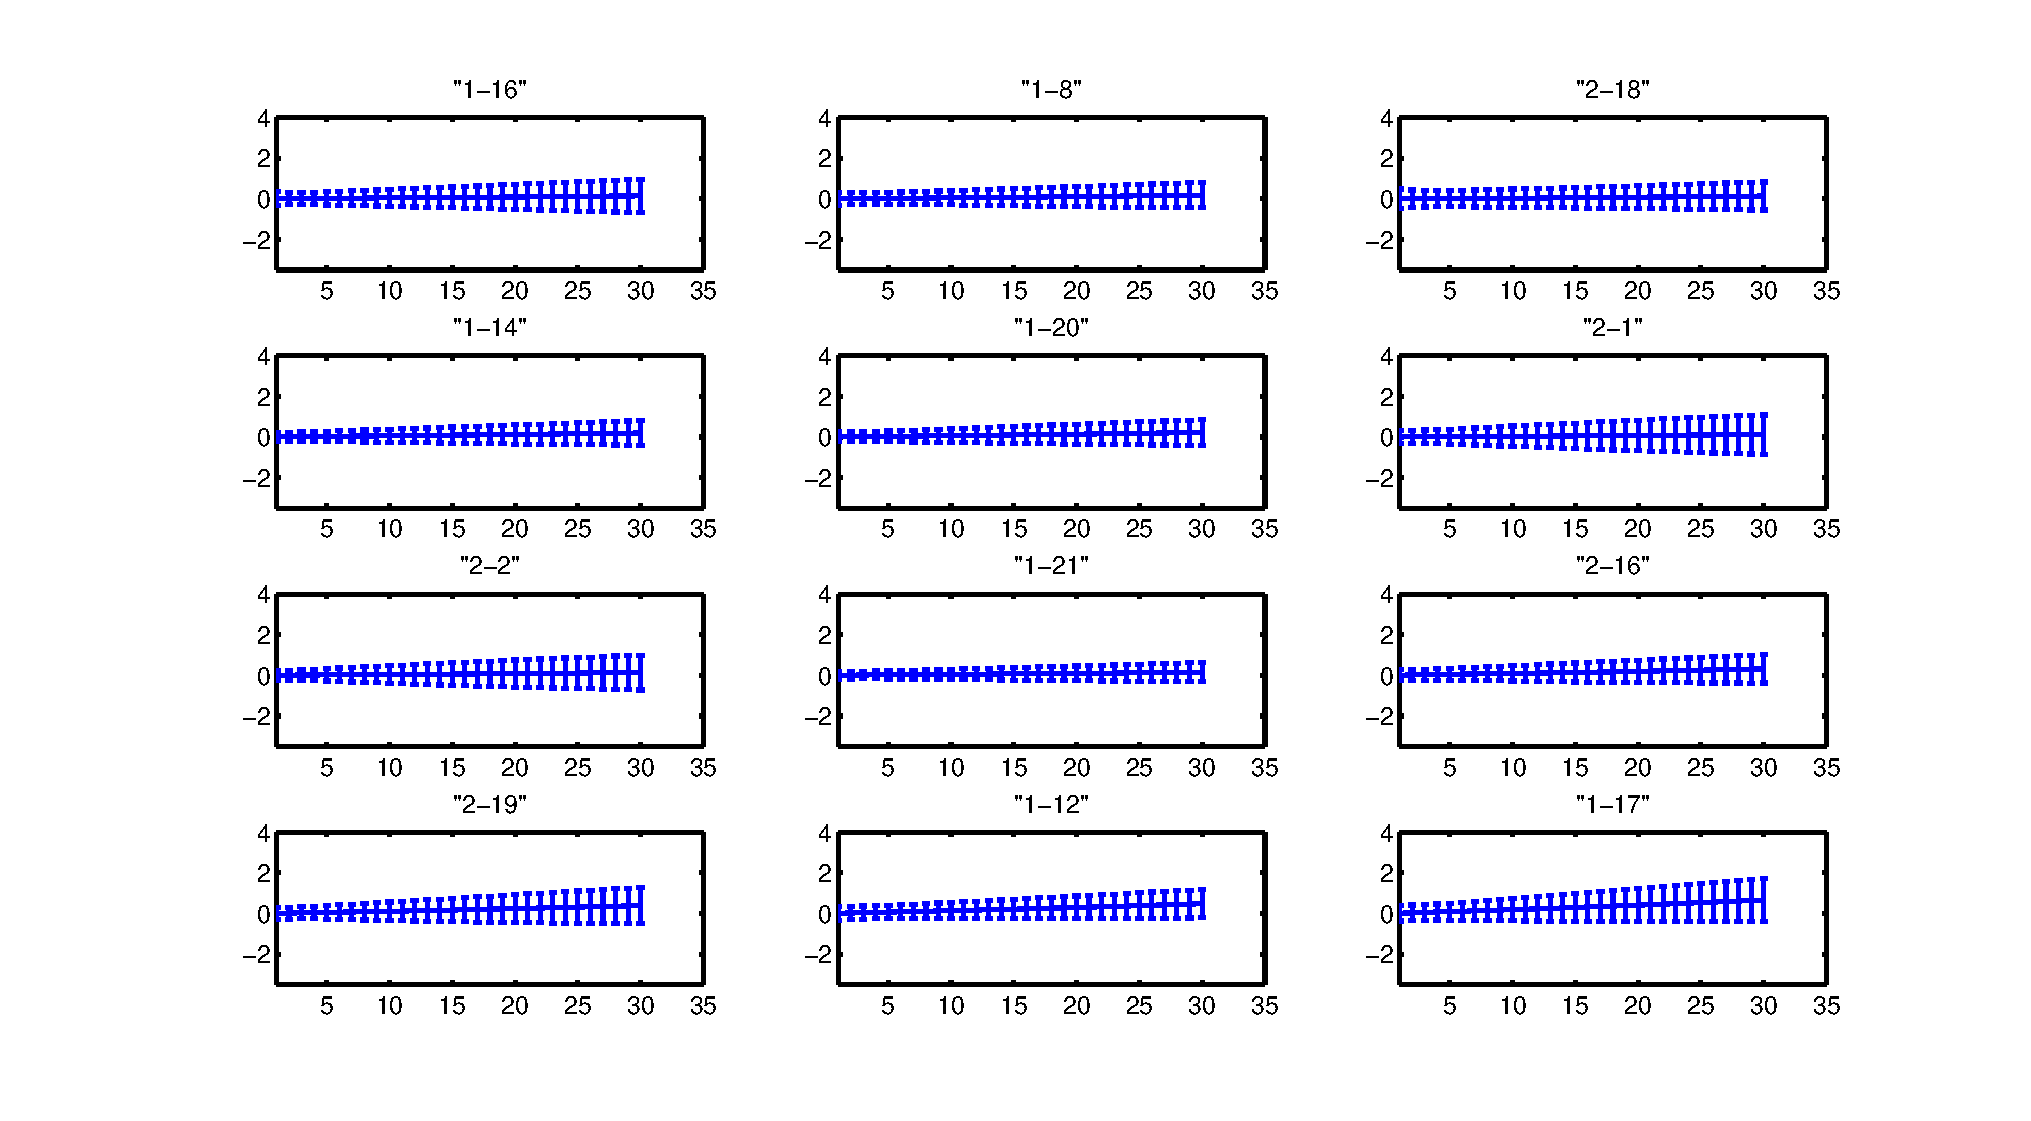
\includegraphics[width=0.8\columnwidth]{fig/PooledSingleError.eps}
\end{center}
\caption[Error distributions for the static $\alpha$ model]{Error distributions
for the static $\alpha$ model, up to 30 minutes into the future. The locations
of the twelve sensors are presented in Figure~\ref{fig:cs1Floorplan}}
\label{fig:staticerror}
\end{figure}

\begin{figure}[!htb]
\begin{center}
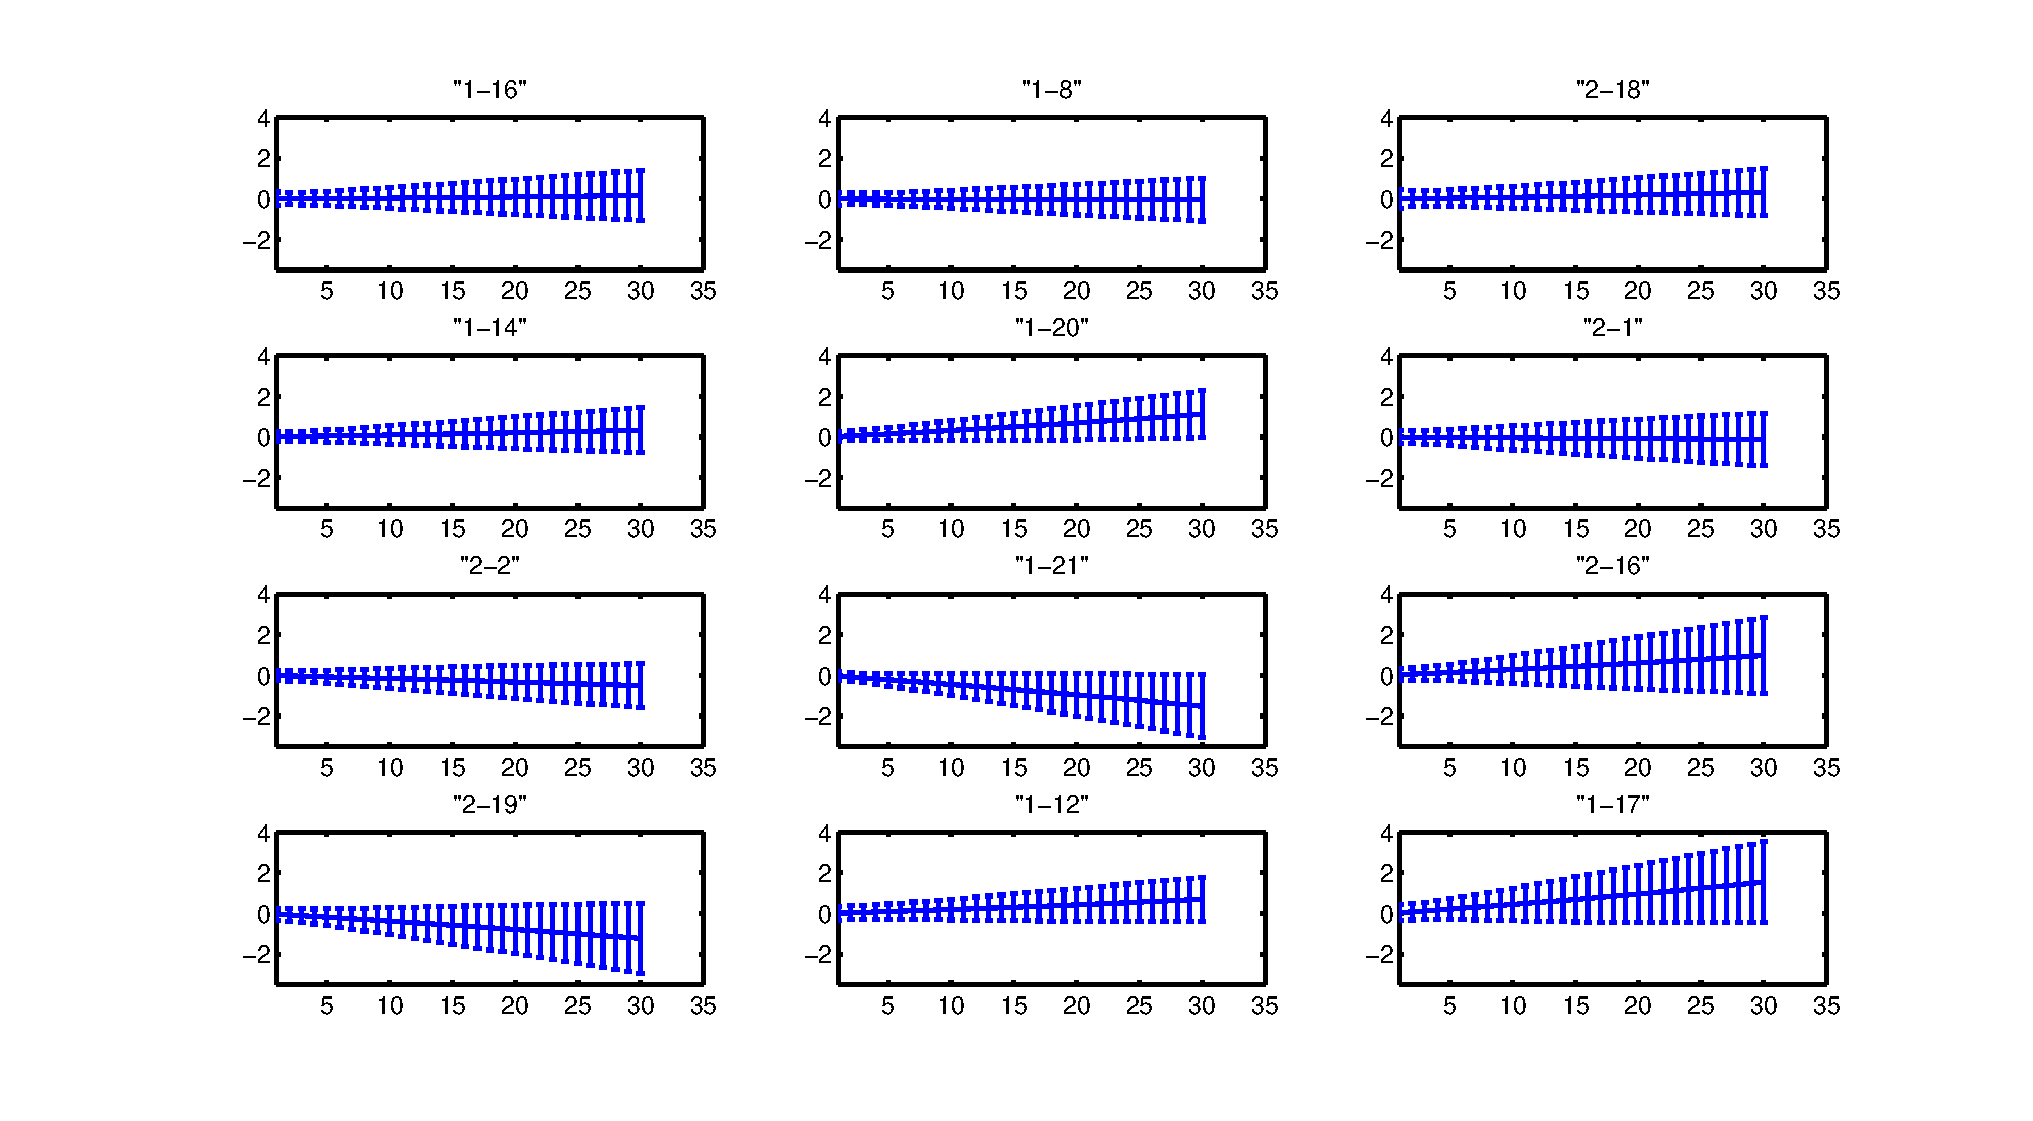
\includegraphics[width=0.8\columnwidth]{fig/DynSingleError.eps}
\end{center}
\caption[Error distributions for the dynamic $\alpha$ model]{Error distributions
for the dynamic $\alpha$ model, up to 30 minutes into the future. The locations
of the twelve sensors are presented in Figure~\ref{fig:cs1Floorplan}}
\label{fig:dynamicerror}
\end{figure}

\begin{figure}[!htb]
\begin{center}
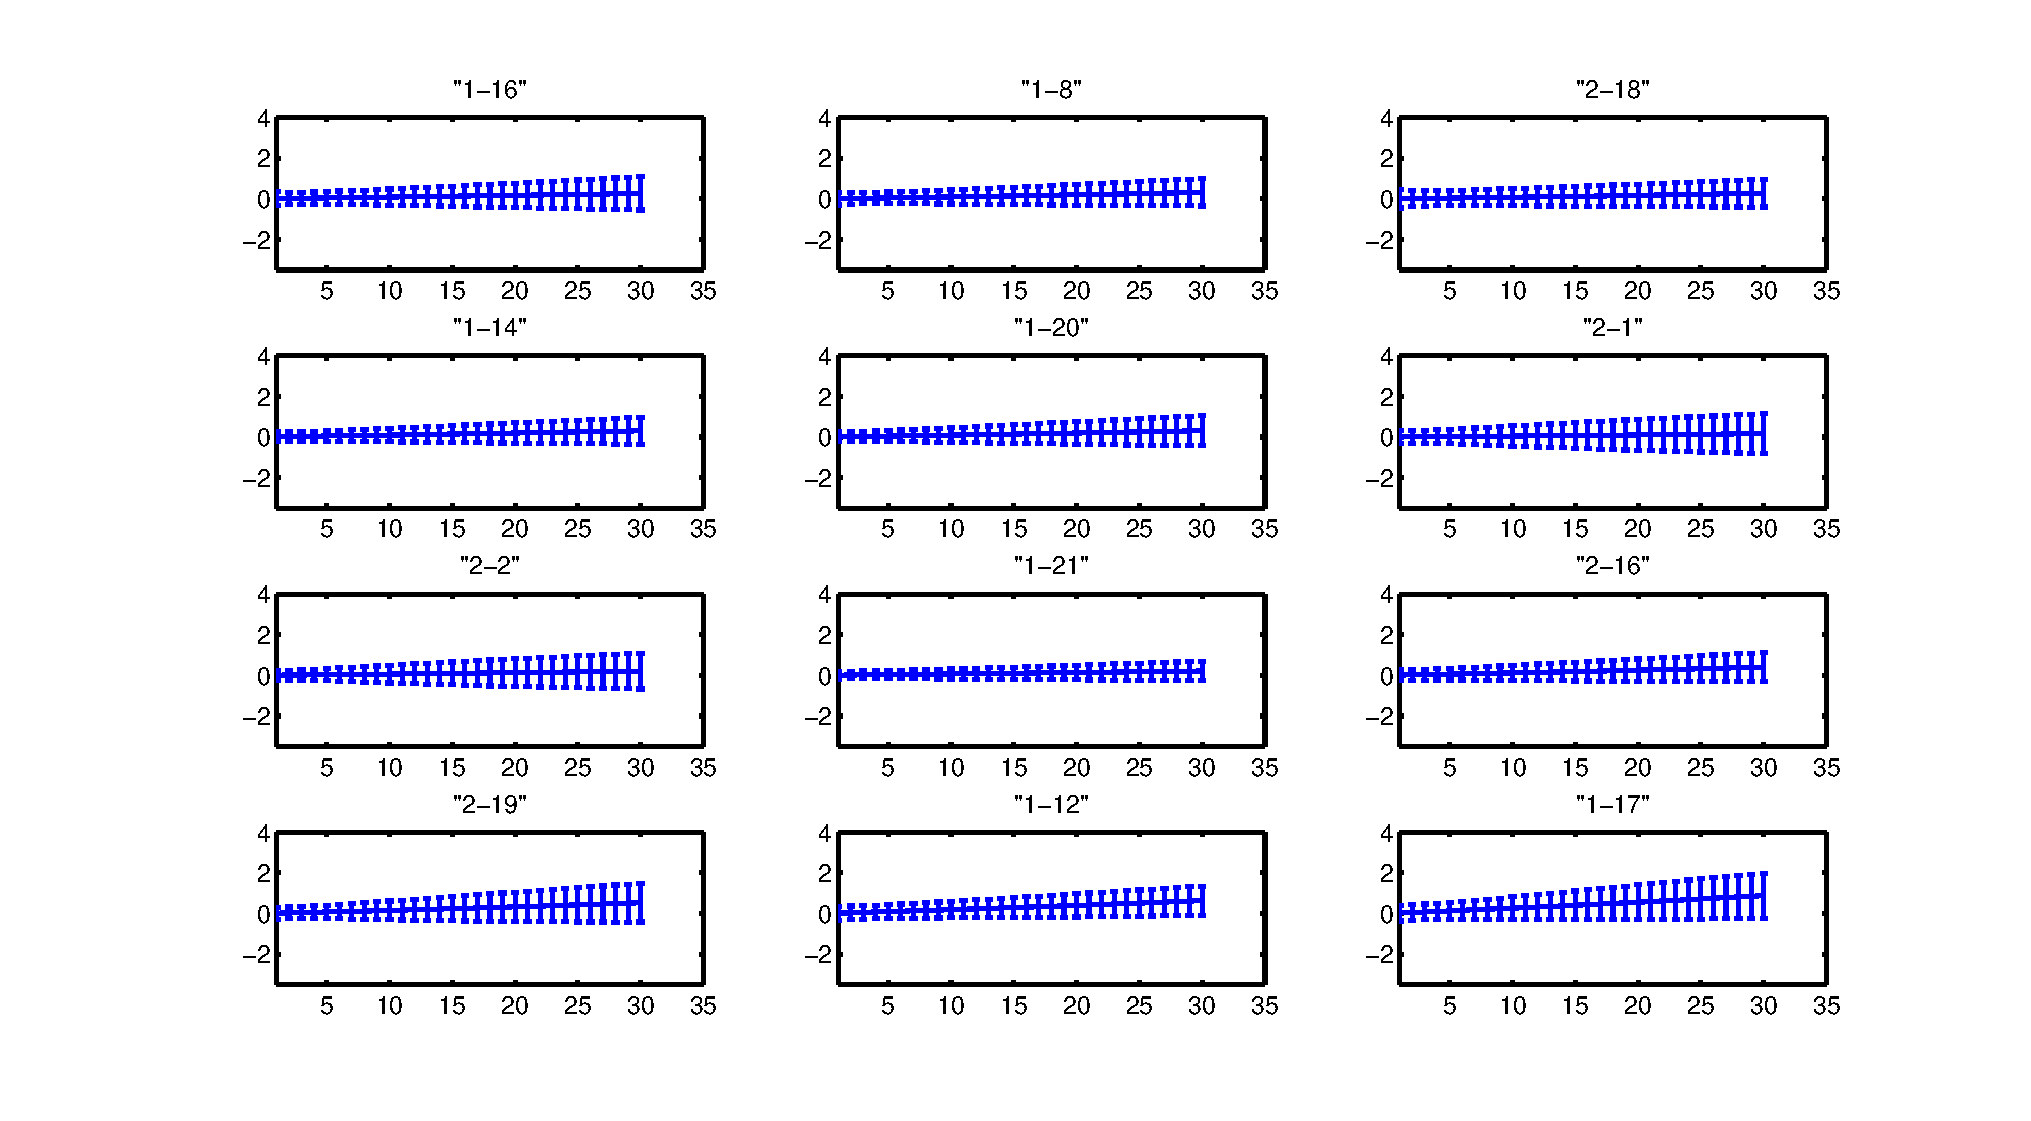
\includegraphics[width=0.8\columnwidth]{fig/PooledAdjError.eps}
\end{center}
\caption[Error distributions for the adjacency model]{Error distributions for
the adjacency model, up to 30 minutes into the future. The locations of the
twelve sensors are presented in Figure~\ref{fig:cs1Floorplan}}
\label{fig:adjerror}
\end{figure}

The error metric chosen for the evaluation is to determine the distribution of
prediction error as predictions are made $t$ minutes into the future. For each
minute, $t$, the mean and standard deviation of the prediction errors $t$
minutes away from the initial time are calculated. The results from these
analysis for the static $\alpha$, dynamic $\alpha$, and adjacency model are
shown in Figure~\ref{fig:staticerror}, Figure~\ref{fig:dynamicerror}, and
Figure~\ref{fig:adjerror} respectively. These results are calculated on a
per-sensor basis for each of the 12 sensors in the 7 rooms of the building.

Visually examining the error distributions highlights a few important things
about the model. The first observation is that variance of the errors tend to
increase as predictions are made further into the future. The error can get
quite large in some places, particularly in the dynamic $\alpha$ model. However,
most of the values for each model remain within 2 degrees for the 30 minute
prediction. This is a reasonable interval with which to enable the control of a
predictive zoning system.

The results from this analysis also indicate that the simple, pooled $\alpha$
model performs better than the dynamic model. This may be counterintuitive since
weather tends to change significantly throughout the day. However, because of
the window being looked at and the narrow range of temperature changes, it is
reasonable that this model should perform well. It also has the added benefit of
being computable and easy to implement within a control setting.

\subsection{Conclusions}
\label{sec:conclusions}

This section presented a model that can be used for thermal prediction in a
zoned HVAC system. The two-stage, dynamic model presented provides an accurate
way to predict the temperature in a zone based on a few, accessible parameters
in the system. It also allows the calculation of highly variable terms, such as
the heat load due to solar radiation, wind, and cloud coverage, without the need
to explicitly measure these terms. This model can be used to implement the
predictive zoning controller. The model provides better insight into the
dynamics of the control scheme and allows for a more efficient design.

\section{Predictive Occupancy Model}
\label{sec:occupancyModel}

% Context and Motivation
% - smart building applications
% - Large number of features 
% -- More features: More accurate, but longer training time
% -- Fewer features: Less accurate, but shorter training time
% - Do not know which features are noisy

In order for room occupancy to be predicted, accurate models of occupancy are
needed. This accuracy usually depends on the granularity of the model where a
very {\em fine-grained model} that captures a large number of features is more
accurate than a {\em coarse-grained model} composed of fewer features.  There
are many features, such as the current state of the room for which a prediction
is required, the states of neighboring rooms, the time of day, etc., that can be
considered when making occupancy predictions. Using all possible features to
make a prediction is impractical due to the large amount of data necessary to
train such a model. Thus, a fine-grained model would be unusable for a long
period of time until sufficient data is collected for it to be useful.  Making
such a system usable in a home might require months, if not years, of training
data collection. Thus, a trade-off has to be made between accuracy and training
time. The traditional approach is to identify the features with the greatest
predictive power and use only them to build an occupancy model. Yet, selecting
these features is not straightforward due to the difficulty of separating noisy
features from those that are highly correlated with occupancy. Furthermore,
every house is different and, thus, a model composed of a single set of features
would not prove accurate across all houses. They also vary within a home
depending on the context. For instance, certain rooms such as the living room
and kitchen are used very frequently and thus a model with many features can be
built within a relatively short period of time, but a room such as the laundry
room, may be used infrequently and thus a more general model, with fewer
features, maybe necessary to be usable within a short period of time.

SmartZone uses a hierarchical model, called {\em Percolator}, to predict the
room-level occupancy in homes. In this section we describe the implementation of
Percolator and evaluate its performance. Percolator can predict occupancy with
accuracies sufficient for most smart home applications. A feature of Percolator
is its ability to automatically increase in accuracy as more data is collected
during the usage of the system. Using a hierarchy of models with various sets of
features also has the added benefit of allowing models to be selected that match
room usage patterns. This would allow fine-grained models to be built quickly
for rooms that are frequently coarse-grained models can be trained for rooms
that are infrequently used. These attributes of a hierarchical model makes
Percolator ideal for the many smart home applications that require the occupancy
of rooms to be predicted with a minimal training period.


% Problem definition: Occupancy predictor that works well within a short period
% of time, but improves in accuracy over time 
% How many training days satisfy criteria?
% Formal definition: State composed of K features and N training days. Decide on
% features to be used to make predictions.

What most smart home systems require is an occupancy predictor that is
sufficiently accurate within a couple of weeks of the system being installed,
but improves in its predictions using the data collected as the system operates
over time. One approach to implement such a predictor is to define a model
composed of a large number of features, but uses only a few of its features to
make predictions initially. Over time, as more data is collected, additional
features are activated. The problems that have to be solved to implement such a
system is deciding when to activate another feature and the order in which the
features should be activated.

% Approach: Hierarchical set of models with decreasing specificity
% Rare states -> General Model
% Frequent states -> Specific Model

% Summary of results

Percolator addresses these problems by utilizing a hierarchical occupancy
prediction approach that uses a set of models ranging from general models, with
few features, to specific models with many features, and automatically selects a
model to make the most accurate prediction possible for a particular
situation. The main benefit to the Percolator approach is the ability for a
smart home application to be able to predict occupancy with over 80\% accuracy
within ten days of being deployed with the prediction accuracy increasing the
longer the system is deployed.

\subsection{Background and Related Work}
\label{sec:occupancyBackground}

% Define in terms of our notation
% Pre-heat
% Smart thermostat
% Neurothermostat
% DGQL
% Sensor Belief Networks

The Neurothermostat~\cite{mozer1997neurothermostat} uses a hybrid occupancy
predictor that leverages a daily schedule and a neural network. Yet, it needed
to be trained on five consecutive months of data to predict occupancy
accurately. The reliance of this approach on a daily schedule and almost half a
year's worth of occupancy data make it infeasible for most smart home
applications. Krumm et al.~\cite{krumm2011learning} present an occupancy
prediction algorithm that gives the probability of occupancy at different times
for each day of the week. This approach would work well for households where the
residents have very similar occupancy patterns for a particular day of the week,
but is unable to respond to changes in occupancy patterns for a particular day.

The DGQL Occupancy Prediction Model (DOPM) is an occupancy prediction model
built using the Decision Guidance Query Language (DGQL)~\cite{5718556}. Its aims
are to maximize energy saved in a location while limiting the inconvenience
caused to its occupants. DOPM is based on presenting prediction rules, which it
then refines using motion sensor data by maximizing the total empty time and
attempting to limit the number of errors to fewer than $n$ where $n$ is an
acceptable inconvenience. A shortcoming of DOPM is that it relies heavily on the
prediction rules. Therefore, providing it with insufficient, or incorrect, rules
could result in inaccurate predictions.

The Smart Thermostat~\cite{Lu2010} uses a Hidden Markov Model (HMM) to predict
occupancy at the house-level. This approach was not evaluated for room-level
occupancy prediction but would necessitate a large amount of data to train an
HMM per room. The HMM approach is similar to other approaches that use Bayesian
probability theory to predict occupancy. Page et al.~\cite{page2008generalised}
use a generalized stochastic model to simulate occupancy presence as an input
for future occupant behavior models within building simulation
frameworks. Dodier et al.~\cite{dodier2006building} use sensor belief networks
in order to detect occupancy. The belief network was used to generate a
probability distribution of occupants and their locations over time given
historical sensor data. Yet, this approach also suffers from requiring a large
amount of training data to provide useful predictions for smarthome
applications.

The latest approach at using occupancy prediction for thermostatic control is by
PreHeat~\cite{scott2011preheat}. Occupancy is detected using RFID tags placed on
house keys to sense if the house is occupied and motion sensors in each room to
sense room occupancy. Occupancy is recorded as a binary vector for each day
where each element of the vector represents the occupancy in a 15 minute
interval with 1 indicating the room was occupied and 0 indicating the room was
vacant. PreHeat predicts the next time a room will be occupied by searching for
the five closest matching days to the current day based on hamming distance and
then calculating the mean of the occupancy values for these days. PreHeat was
implemented in three homes in the United States and two homes in the United
Kingdom. Leveraging the room-level radiators and underfloor hearing units
commonly used in the UK, PreHeat provides room-level heating control. The
implementation of PreHeat in the United States resorted to controlling the HVAC
system based on whole house occupancy due to HVAC systems in the US
traditionally being centralized units. PreHeat works well for homes with regular
occupancy patterns, but would not work as well for homes where the occupants do
not have regular schedules. The method also requires a large amount of
historical data in order to find five days with occupancy patterns closely
matching any given day.  The main weakness of PreHeat that Percolator attempts
to address is the lack of interaction between rooms in any of the models used
for prediction. For instance, the authors predict the occupancy of each room
based on the history of occupancy of that particular room without considering
the occupancy of any other rooms. Taking into consideration occupancy patterns
across a house would lead to higher accuracies in predicting the occupancy of a
particular room. The authors also use a very simple thermal model to predict
when a room should be preheated. The model is simply the average amount of time
it took to increase the room temperature by a degree based on historical
data. Predictive zoning uses a model that takes into consideration the thermal
interactions between rooms. Also, PreHeat does not provide a room-level solution
for houses with centralized HVAC systems which RoomZoner and Smart Zone
provide. 

\subsection{Approach}
\label{sec:occupancyApproach}

% Percolator model
% - Description of models and submodels
% - Description of decision procedure
% - Description of fallback

Percolator is composed of a set of {\em predictors}: occupancy models built from
historical occupancy data showing how many times a particular set of features
has been observed in the past, the {\em total observation count}, and how many
times a room has been occupied when these features were observed, the {\em room
occupancy count}. These counts are for various {\em prediction horizons}: times
into the future for which predictions are desired. In the implementation
presented in this section, prediction horizons of 1 minute, 2 minutes, 3
minutes, 5 minutes, 10 minutes, 20 minutes, and 30 minutes are
used. Table~\ref{table:curTimePredictor} shows an example of a simple predictor
that uses only the current time as the feature.

\begin{table}[!htb]
  \caption{Example of a predictor with current time as feature.}
  \centering
  \begin{tabular}{| l | c | c | c | c | c |}
    \hline
    Time & Room 1 @ 1 min & Room 1 @ 2 min & ... & Room N @ 30 min & Total Observations\\ \hline
    00:00 & 5 & 0 & 15 & 1 & 30 \\ \hline
    00:01 & 4 & 1 & 20 & 5 & 31  \\ \hline
    00:02 & 1 & 3 & 22 & 0 & 30 \\ \hline
    ... & ... & ... & ... & ... & ... \\
    \hline
  \end{tabular}
  \label{table:curTimePredictor}
\end{table}

In Percolator the predictors are composed in a hierarchical manner ordered from the most
fine-grained predictor to the most coarse-grained
predictor. Figure~\ref{fig:percolatorExample} illustrates an instance of
Percolator with a {\em percolation depth}, the number of predictors composing
the model, of two. As the arrows indicate, Percolator is ordered from
fine-grained predictors to coarse-grained predictors. Also, a smaller percentage
of all possible feature combinations would have been observed for a fine-grained
model than a coarse-grained model because there are more possible combinations
for a fine-grained model. 

\begin{figure}[!htb]
\begin{center}
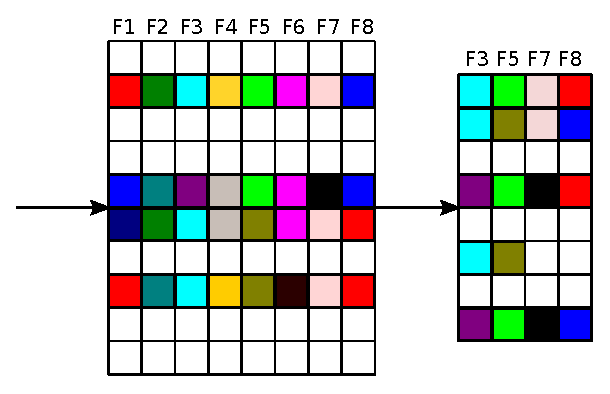
\includegraphics[width=0.6\columnwidth]{fig/percolatorExample.eps}
\end{center}
\caption[Illustration of a Percolator model instance]{An illustration showing an
instance of Percolator composed of two predictors. The first predictor is
composed of eight features ($F1$ - $F8$) while the second predictor is composed
of a subset of four of these eight features. Filled rows indicate a particular
combination of features that has been observed while empty rows indicate feature
combinations that have not yet been observed. The colors illustrate the values
that the feature could take. For instance, if the feature is room state, the
colors indicate occupied or vacant. This figure only illustrates feature
combinations. In Percolator, each feature combination has an associated room
occupancy count and total observation count as shown in
Table~\ref{table:curTimePredictor}.}
\label{fig:percolatorExample}
\end{figure}

Figure~\ref{fig:observationExample} illustrates an observation of the eight
features for which an occupancy prediction in the future is desired. There is no
row in the fine-grained predictor that matches this combination of
features. Therefore, Percolator percolates the prediction decision to the next
predictor in the hierarchy. In this instance, features 3, 5, 7, and 8 that are
observed match the second row of the coarse-grained predictor and therefore the
room occupancy count, $C_R$, for the room and prediction horizon, $k$, of interest and
total observation count, $C_T$, associated with this set of features is obtained
from this predictor. The probability of occupancy, $P_O$, is calculated as $P_O
= C_R / C_T$. If this fraction is greater than an {\em occupancy threshold} the
room is predicted to be occupied $k$ minutes in the future.

\begin{figure}[!htb]
\begin{center}
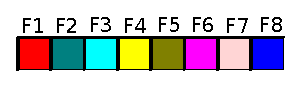
\includegraphics[width=0.4\columnwidth]{fig/observationExample.eps}
\end{center}
\caption[Illustration of observed feature set]{An illustration of a set of
observed features. These observed features can be used to make a prediction of
future occupancy using Percolator.}
\label{fig:observationExample}
\end{figure}

Making a prediction based on a few prior observations could result in incorrect
predictions being made. In order to minimize such occurrences, Percolator uses a
{\em percolation threshold}: the minimum number of observations on which a
prediction can be made. If the total observation count is below the percolation
threshold, the prediction decision is percolated up the hierarchy. As more
observations are expected with coarser-grained predictors, percolating up the
hierarchy increases the probability of using a predictor that satisfies the
percolation threshold.

In the event that none of the predictors in the hierarchy has sufficient
historical data to make a prediction, Percolator has a number of fall-backs it
can use to make a prediction. The most simple of these fallback techniques is
{\em current state} where the model simply predicts that the room would simply
remain at its current state, whether occupied or unoccupied. Another fallback
technique evaluated is {\em hamming distance} where, in the event Percolator
cannot find sufficient historical days even with the most general model, it
looks for the day with the set of features closest to the currently observed
feature set based on hamming distance and use the observed occupancy of the room
at that day as the prediction. This method proved too computationally intense to
be practical, and therefore {\em current state} was selected as the fallback for
Percolator.

% Each occupancy predictor searches through historical occupancy data for all
% instances with identical features to those currently observed. The
% implementation of Percolator used current time and room states as features, but
% additional features such as day of the week, whether it is a weekend or a week
% day, etc. can be used to build additional predictors. Once these historical
% days, which share the currently observed features, are found Percolator looks
% $k$ minutes into the future of the room $r$ for which a prediction is
% needed. For instance, if the current time is 9:00 AM and a prediction of room
% occupancy at 9:15 AM is needed for the living room, Percolator would look at the
% occupancy of the living room at 9:15 AM for all days which had the same set of
% features at 9:00 AM as today. The probability of occupancy is, then, calculated
% by dividing the number of times the room was observed to be occupied at this
% time by the total number of days which shared the current feature set. If this
% probability is greater than an {\em occupancy threshold} the room is predicted
% to be occupied. Otherwise, the room is predicted to be unoccupied.

% Percolator first uses the model at the bottom of the percolation tree, which has
% the most features and, thus, is potentially the most accurate, to make a
% prediction. If the number of historical days found with all features matching is
% fewer than a {\em percolation threshold}, the prediction is percolated up the
% tree to a less specific model. This process continues until a predictor for
% which a sufficient number of historical days matching the currently observed
% features is found, and this predictor is used to make a prediction. This
% approach is based on the intuition that a more detailed model is more likely to
% make an accurate prediction, yet would require a large amount of data to
% encapsulate all combinations of features. Thus, when the model is first deployed
% more general occupancy predictors, such as the one that uses only the current
% time, would be used to make a prediction, but as the system runs and collects
% more occupancy data, the more specific models can be completed and are more
% likely to be used to make predictions. This would lead to the model becoming
% more accurate over time.

\subsection{Experimental Setup}
\label{sec:occupancyExperiment}

% Describe four houses and sensor deployments

\begin{table}[!htb]
\centering
\begin{tabular}{|c|c|c|c|c|c|}
\hline
  \small \#Residents & \small \#Rooms & \small \#Motion & \small \#Weeks \\
  & & \small Sensors & \\
\hline
 \small 2 & \small 7 & \small 14 & \small 12 \\
 \small 1 & \small 7 & \small 8 & \small 24 \\
 \small 2 & \small 10 & \small 10 & \small 8 \\
 \small 3 & \small 7 & \small 7 & \small 12 \\
\hline
\end{tabular}
\caption{Details of the 4 homes from which occupancy data was collected}
\label{table:deploymentDetails}
\end{table}

Data collected from four residences over periods ranging from two to six months
was used to evaluate Percolator. These deployments included both single- and
multi-person homes with varying occupancy patterns. The residents ranged from
students and working professionals to stay at home parents and residents who
worked at home. Table~\ref{table:deploymentDetails} summarizes the information
about the homes. Ten-fold cross-validation is used to train and test the model
using the collected occupancy data to generate the results presented in
Section~\ref{sec:occupancyResults}.  Figure~\ref{fig:percolatorModel} shows the
prediction hierarchy used for the evaluation.

\begin{figure}[!htb]
  \centering
  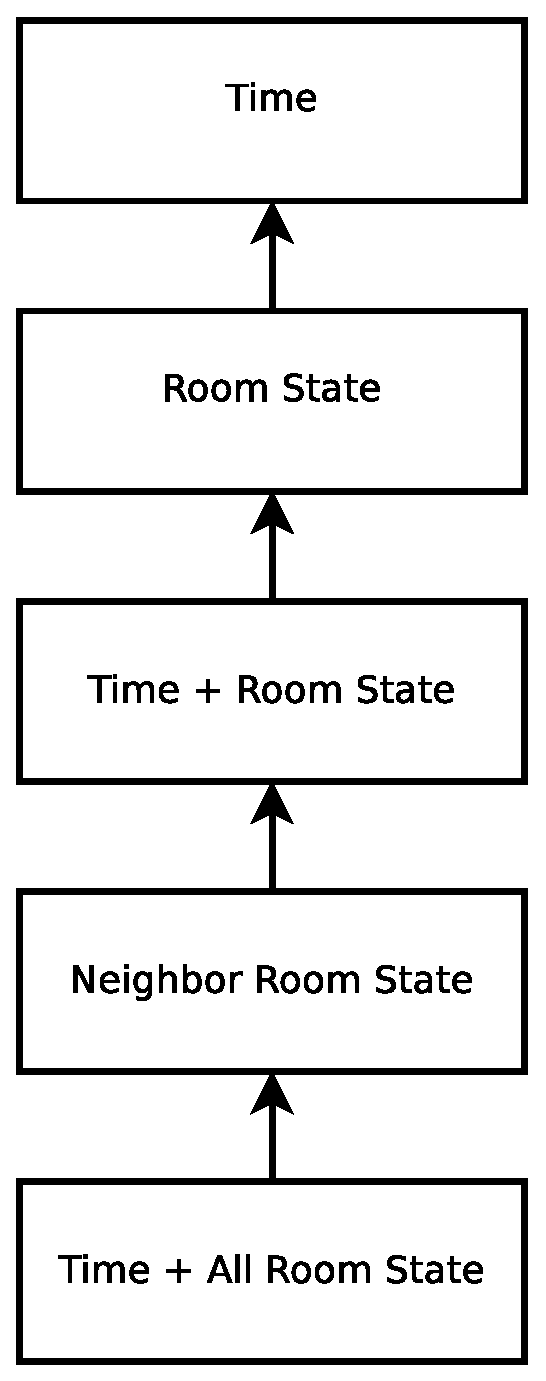
\includegraphics[width=0.3\columnwidth]{fig/percolator.eps}
  \caption[Percolator Occupancy Model]{The Percolator hierarchical occupancy
  predictor starts at the bottom of the hierarchy with the most specific, and
  accurate, occupancy model and percolates up towards more general models until
  a perfect match of features is found.}
  \label{fig:percolatorModel}
\end{figure}

\subsection{Results}
\label{sec:occupancyResults}

The performance of Percolator is evaluated across the four houses as the amount
of training data available increases. As
Figure~\ref{fig:trainingSetSizeAccuracy} shows, Percolator achieves over 75\%
accuracy within 10 days of deployment with accuracy increasing as it is trained
with more data.

\begin{figure}[!htb]
\begin{center}
\includegraphics[width=0.6\columnwidth]{fig/accuracy4Houses.eps}
\end{center}
\caption[Accuracy of Percolator as more training data is available]{Percolation
increases in accuracy with more training data achieving over 75\% accuracy
across all four houses with only 10 days worth of data.}
\label{fig:trainingSetSizeAccuracy}
\end{figure}


\subsection{Sensitivity Analysis}
\label{sec:sensitivityAnalysis}
Sensitivity analyses are performed to understand how varying the parameters
associated with Percolator affects its performance.

\subsubsection{Training Set Size}

Figure~\ref{fig:trainingSetSizeVsPredictorSelection} shows the effect on the
accuracy as Percolator is trained with more data. Maintaining the sensitivity
threshold at 3 and increasing the size of the training set from 10 days worth of
data to 60 days of data results in an accuracy increase from 74\% to 83\%. This
increase in accuracy is due to more decisions being made with the more accurate
fine-grained predictors as more data is available to train the model. At most
training set sizes Percolator outperforms the component predictors by
efficiently selecting between them to make an accurate prediction. Also, as
expected the accuracy of Percolator increases as more data is available for
training.

\begin{figure}
\centering{
\subfigure[House 1]{
\includegraphics[width=.45\columnwidth,height=.45\columnwidth,keepaspectratio=true]{./fig/trainingSetAccuracy_houseA}
\label{fig:houseA_accuracy}
}
\subfigure[House 2]{
\includegraphics[width=.45\columnwidth,height=.45\columnwidth,keepaspectratio=true]{./fig/trainingSetAccuracy_houseB}
\label{fig:houseB_accuracy}
}
\subfigure[House 3]{
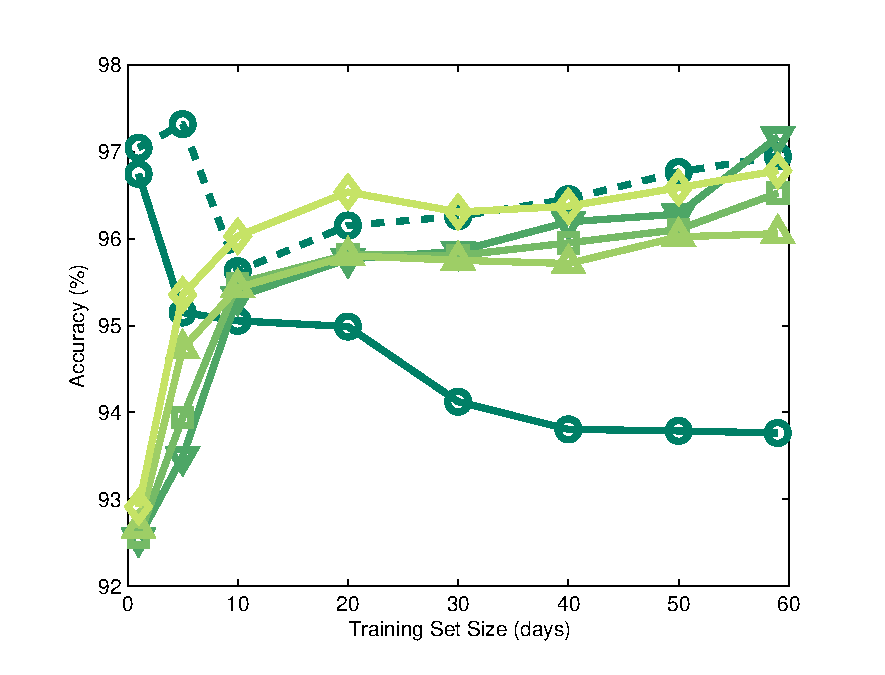
\includegraphics[width=.45\columnwidth,height=.45\columnwidth,keepaspectratio=true]{./fig/trainingSetAccuracy_houseE}
\label{fig:houseE_accuracy}
}
\subfigure[House 4]{
\includegraphics[width=.45\columnwidth,height=.45\columnwidth,keepaspectratio=true]{./fig/trainingSetAccuracy_houseF}
\label{fig:houseF_accuracy}
}
\caption[Accuracy of Percolator compared to its component predictors]{Percolator
achieves over 65\% accuracy in predicting rooms to be occupied in all four
houses with two months of training data. Three of the four houses achieve
over 75\% accuracy with only 20 days of training data.}
\label{fig:trainingSetSizeVsPredictorSelection}
}
\end{figure}

Figure~\ref{fig:trainingSetSizeModelUsage} also shows that the predictor with
the greatest accuracy varies from house to house and as more data is
collected. For instance, in House 1 with 20 days of training data the most
accurate predictor is the one that uses the current time and states of all the
rooms as the prediction features while for House 2, with the same amount of
training data, the predictor that uses only the neighboring room states is the
most accurate. Also, with less training data coarse-grained predictors such as
those that use only the state of the room of interest is more accurate than
finer-grained predictors, but as more data is collected the finer-grained
predictors become more accurate than the coarse-grained predictors.

% \begin{figure}[h]
% \begin{center}
% 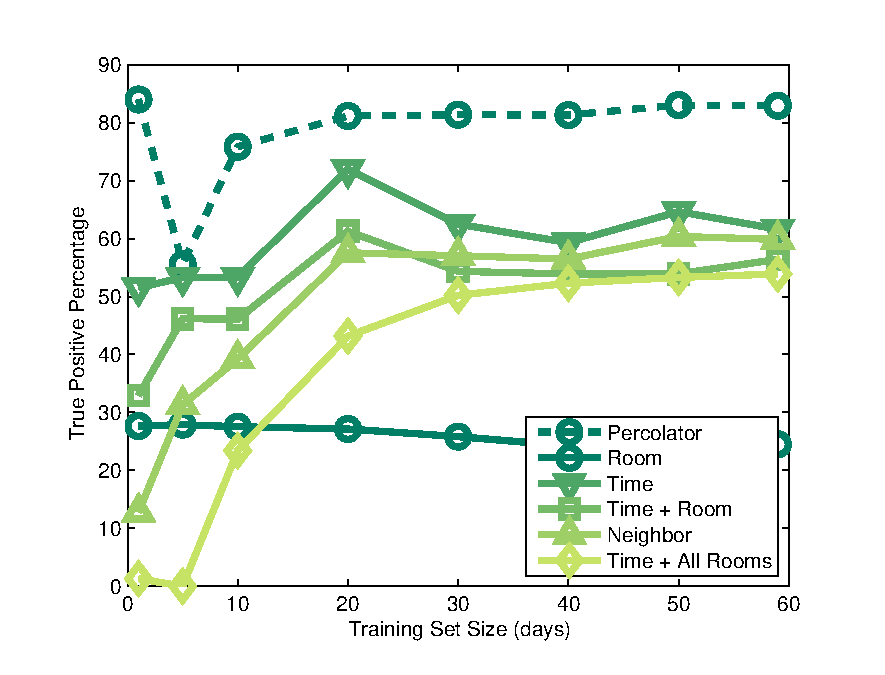
\includegraphics[width=0.6\columnwidth]{fig/trainingSetSizeModelType.eps}
% \end{center}
% \caption[Sensitivity of Percolator to the training set size]{Percolation is more
% accurate than all of the predictors at all training set sizes. With only a few
% days of data to train with, simpler predictors that use features such as the
% current room state are more accurate than more specific predictors that use many
% features such as the time and the state of all rooms or the state of neighboring
% rooms, but as more data is available for training the specific predictors become
% more accurate than the simpler general predictors.}
% \label{fig:trainingSetSize}
% \end{figure}

\begin{figure}[!htb]
\begin{center}
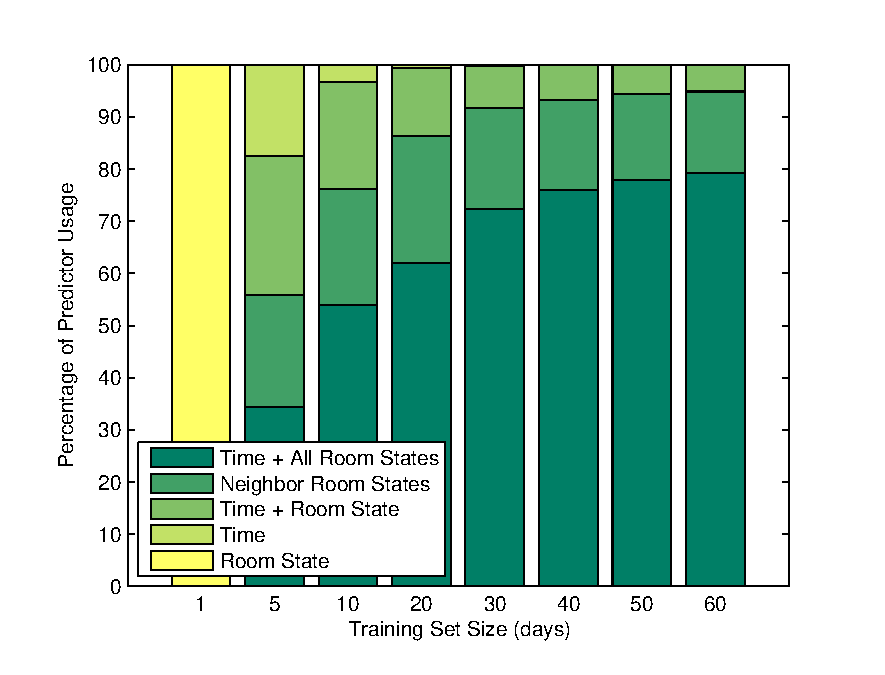
\includegraphics[width=0.6\columnwidth]{fig/trainingSetSizeModelUsage.eps}
\end{center}
\caption[Effect of training set size on predictor selection]{As the training set
size increases, a greater fraction of the decisions are made using the more
specific predictors.}
\label{fig:trainingSetSizeModelUsage}
\end{figure}

\subsubsection{Prediction Horizon}

As with most models that attempt to make predictions, Percolator gets less
accurate as it makes predictions further into the future from the current
time. Figure~\ref{fig:predictionHorizon} shows the effect on the accuracy across
the four houses as this {\em prediction horizon} increases from one minute in
the future to 30 minutes into the future. With only 60 days of training data,
occupancy could be predicted with about 60\% accuracy 20 minutes into the future
and for shorter prediction horizons over 90\% accuracy is possible. This
accuracy is expected to increase as more training data is available.

\begin{figure}[!htb]
\begin{center}
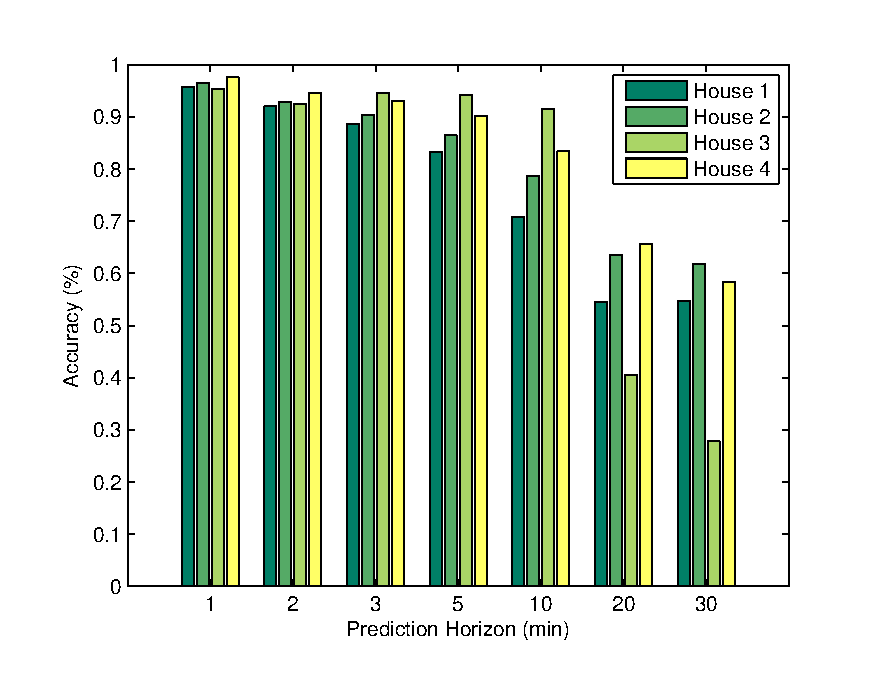
\includegraphics[width=0.6\columnwidth]{fig/predictionHorizonAccuracy.eps}
\end{center}
\caption[Sensitivity of Percolator to the prediction horizon]{The average
accuracy of predictions across the four house drops from 96\% to 51\% as the
prediction horizon increases from one minute to 30 minutes.}
\label{fig:predictionHorizon}
\end{figure}

Figure~\ref{fig:predictionHorizonModelType} shows the effect of increasing the
prediction horizon on the five predictors that compose Percolator. Percolator
does better than all predictors until a prediction horizon of 10 minutes. Beyond
that horizon, it does as well as the neighbor room state predictor. More
sophisticated algorithms for percolation thresholding are being developed to
transition between predictors and select better predictors at further prediction
horizons. This would enable Percolator to do at least as well as the most
accurate predictor at any prediction distance.

\begin{figure}[!htb]
\begin{center}
\includegraphics[width=0.6\columnwidth]{fig/predictionHorizonModelType.eps}
\end{center}
\caption[Effect of increasing prediction horizon on occupancy predictors]{For
the first house, Percolator does better than all component predictors for short
prediction horizons and performs as well as the predictor with the average
accuracy for horizons further into the future. The solid lines show the five
predictors that compose Percolator, and the dashed line shows the accuracy of
Percolator.}
\label{fig:predictionHorizonModelType}
\end{figure}

\subsubsection{Percolation Threshold}

\begin{figure}[!htb]
\begin{center}
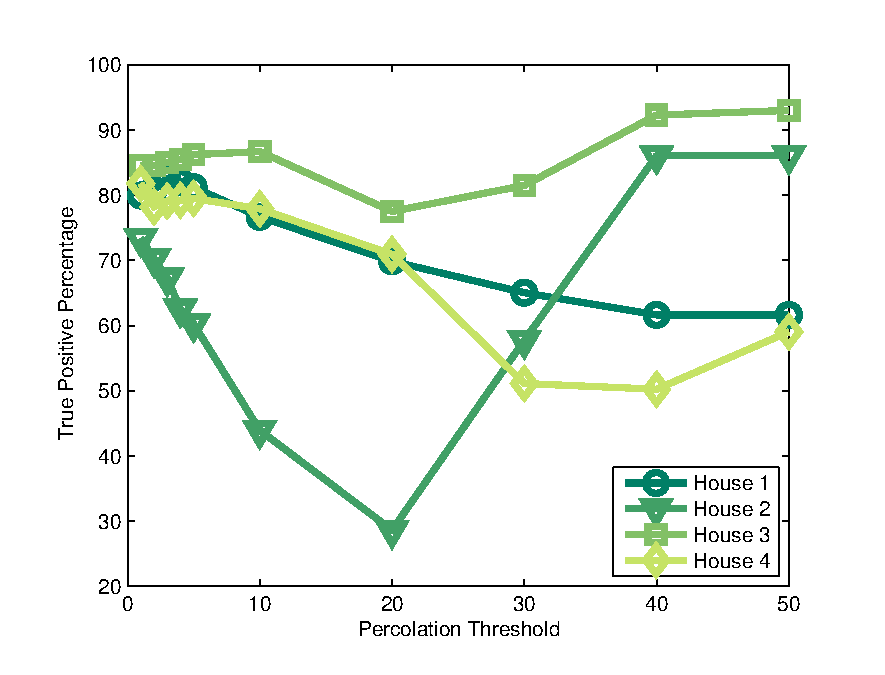
\includegraphics[width=0.6\columnwidth]{fig/percolationThreshold4Houses.eps}
\end{center}
\caption[Sensitivity of Percolator to the percolation threshold]{Prediction
accuracy increases as the percolation threshold increases until the threshold is
too high for the amount of data used to train the model.}
\label{fig:percolationThreshold}
\end{figure}

As described in Section~\ref{sec:occupancyApproach} the percolation threshold is
the minimum number of days with identical features necessary before an occupancy
predictor can be used make a prediction. If the threshold is not met, a less
specific predictor is tried. Figure~\ref{fig:percolationThreshold} shows the
effect of varying the percolation threshold on true positive accuracy for one of
the houses. The model was trained with 60 days worth of data and tested on
another day's worth of data. The graph shows that as the percolation threshold
increases from 1 to 3, the prediction accuracy increases. This is due to the
fact that using more historical data to make a prediction would result in a more
accurate prediction. Yet, a further increase of the percolation threshold, from
3 to 5, causes a drop in accuracy. This is due to 60 days of training data being
insufficient for four or five identical instances to be found for the more
accurate specific predictors, and therefore the decision would percolate up the
hierarchy resulting in a less accurate, more general predictor being used to
make the prediction as shown in
Figure~\ref{fig:percolationThresholdVsModelUsage}.

\begin{figure}[!htb]
\begin{center}
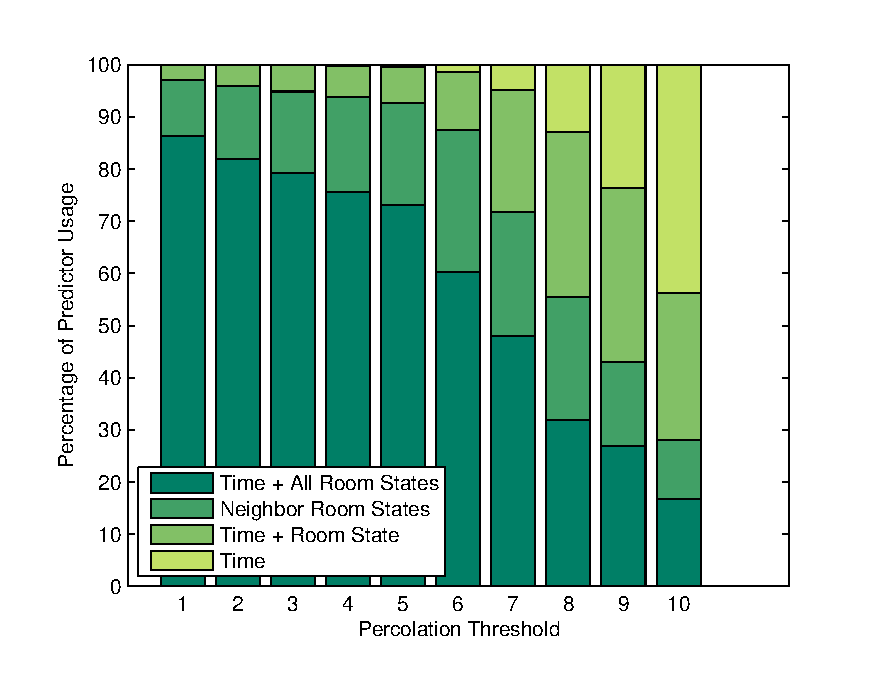
\includegraphics[width=0.6\columnwidth]{fig/percolationThresholdVsModelUsage.eps}
\end{center}
\caption[Effect of percolation threshold on predictor selection]{As the
percolation threshold increases, more decisions percolate up the hierarchy from
specific models towards general models.}
\label{fig:percolationThresholdVsModelUsage}
\end{figure}

\subsubsection{Percolation Depth}
{\em Percolation depth} is the depth of the percolation hierarchy. This is
varied by changing the number of predictors composing
Percolator. Figure~\ref{fig:percolationDepth} shows that adding more models to
Percolator increases its accuracy across all training set sizes. At three models
and 20 days worth of training data Percolator is as accurate as it is with four
or five models. 

\begin{figure}[!htb]
\begin{center}
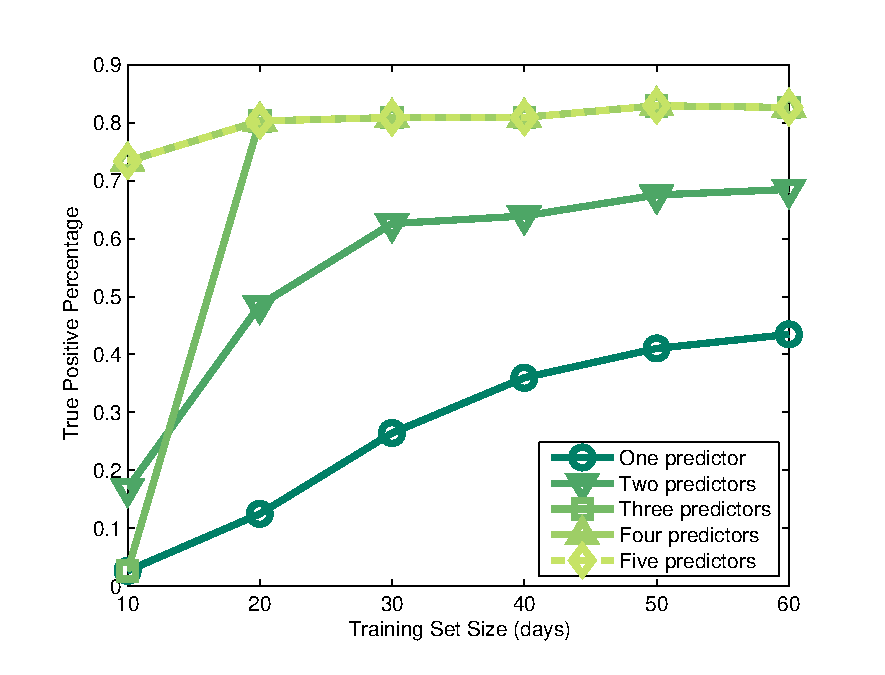
\includegraphics[width=0.6\columnwidth]{fig/percolationDepth.eps}
\end{center}
\caption[Effect of percolation depth on accuracy]{As more predictors are added
to Percolator, the accuracy increases.}
\label{fig:percolationDepth}
\end{figure}

\subsection{Conclusions}
This section presents Percolator, a model that can be used for occupancy
prediction in a zoned HVAC system. Percolator addresses the issue of accurate
occupancy prediction requiring large amounts of data on which to train models,
yet most applications requiring accurate occupancy prediction within weeks of
being deployed. Percolator exploits a hierarchy of occupancy predictors of
decreasing granularity to enable occupancy predictions with over 75\% accuracy
to be achieved within 20 days of a system being deployed. An added benefit of
Percolator is its ability to improve its prediction accuracy as more data is
collected. Thus, over time as the smart home application continues to be used
predictions with greater accuracy would be possible.


\section{Predictive Control}
The predictive thermal model and the predictive occupancy model can be used to
implement SmartZone. One approach for such a predictive zoning controller would
be to optimize over a search space of all possible actuation decisions
attempting to minimize the following cost function:

\begin{equation}
\label{smartzoneCostFunction}
C = \alpha E + \beta M
\end{equation}

\noindent where $E$ is the expected energy expenditure for the control decision
and $M$ is a {\em miss penalty} that captures the discomfort a resident could
expect due to the control decision. $E$ can be calculated as 

\begin{equation}
\label{smartzoneCostFunction}
E = e_s * t
\end{equation}

\noindent where $e_s$ is the energy consumed by a particular HVAC stage and $t$
is the amount of time for which the stage is expected to be active. Percolator
and the predictive occupancy model are used to estimate $M$. Percolator is used
to predict which rooms are occupied from the current time until the next control
decision will be made and the predictive thermal model is used to estimate the
effect of a particular damper configuration and HVAC stage on the temperatures
of those rooms. The total amount of time the rooms are above or below the
setpoint is $M$. $\alpha$ and $\beta$ are wighting functions that can be exposed
to the residents as knobs in order for them to be able to trade-off comfort for
energy savings. By increasing $\alpha$ relative to $\beta$ the residents could
indicate that they are willing to tolerate a longer lag-time in order to save
energy while increasing $\beta$ relative to $\alpha$ would indicate the
residents prioritize their comfort over potential energy savings.

\section{Macroprogramming Discussion}
While SmartZone has not yet been implemented, two of its main components the
predictive temperature and occupancy models were implemented using Matlab and
Python respectively. The Matlab-based occupancy prediction code can be added to
a MacroLab implementation of SmartZone with very minimal, if any, alterations due to
MacroLab supporting all native Matlab functions. The Python implementation of
Percolator heavily relied on the Numpy package which provides Matlab-like
functionality within Python. Therefore, porting this code to MacroLab would
require very little effort. Figure~\ref{code:cs3} shows the high-level logic
implemented in MacroLab.

\begin{figure}[!htb]
  \begin{macrolab}
RTS = RunTimeSystem();
weatherdirect = RTS.getMotes('type', 'weatherdirect');
tempSensors = SensorVector(weatherdirect, 'temperature');
x10 = RTS.getMotes('type', 'X10');
motionSensors = SensorVector(x10, 'motion');
motionSensorIDs = uint8({[8 1 9], [2 6], [10 5], [4], [7 11], [12 14], [3 15]});
tempSensorIDs = uint8({[1 3], [2], [6 7], [4 9 11], [12 13], [5 14], [8 10]}); 
damperIDs = uint8(1:15);
nightStart = [0 0 0 2 0 0];
nightEnd = [0 0 0 7 0 0];
curState = 'On'
every(60000)
  mode = dbRead('zoning', 'mode', 'latest')
  motionVals = motionSensors.sense();
  tempVals =  tempSensors.sense();
  occupancyPrediction = Percolator(motionVals, 1)
  hvacChoices = []
  damperConfigs = []
  costs = []
  for hvacStage = 0:2
    for numClosedDampers = 0:15
      for damperCombination = combntns(damperIDs, numClosedDampers)
        temperaturePrediction = tempPredictor(hvacStage, damperCombination, tempVals)  
        cost = costEstimator(hvacStage, damperCombination, occupancyPrediction,
        temperaturePrediction)
        hvacChoices(end + 1) = hvacStage
        damperConfigs(end + 1) = damperCombination
        costs(end + 1) = cost
      end
    end
  end

  minIndex = find(costs == min(costs))
  optimumStage = hvacChoices(minIndex)
  optimumDamperConfig = damperConfigs(minIndex)
  hvacActuate(mode, optimumStage, optimumDamperConfig)
end
  \end{macrolab}
  \smallskip
  \hrule width 1\columnwidth
  \caption{MacroLab implementation of SmartZone.}
  \label{code:cs3}
\end{figure}

The trend of increasing application complexity decreasing the freedom with which
MacroLab can optimize code implementation continues with SmartZone. While
RoomZoner could benefit from in-network aggregation in larger homes with
multi-hop networks, SmartZone cannot aggregate any sensor values due to all
sensor data being required to train, and improve, the predictive
models. Macroprogramming languages are still beneficial to implementing such
applications due to the simpler programming abstraction they provide over
node-level programming. 

\section{Conclusions}
This case study demonstrates the benefit of an easy to use high-level
programming model to implement a complex CPS application. SmartZone involves all
aspects of the most sophisticated CPS applications: data collection, real-time
computation, actuation, and prediction. Due to all the collected data being
required to train the prediction models, a macroprogramming abstraction does not
have any flexibility to optimize the code implementation. Yet MacroLab greatly
eases the application development process by presenting the programmer an
abstraction of all the data as vectors. The programmer is not burdened with
low-level network details such as sending and receiving messages or handling
dropped packets and instead can focus on writing, and debugging, the application
logic which in itself is a difficult task for such a complicated CPS
application. While SmartZone was not implemented due to such a study requiring
another year of data collection, the major components for its implementation,
the predictive temperature and occupancy models, are evaluated in this
chapter. An overview of an approach to use these models to implement SmartZone
is also presented.

% Individual performance
% Performance of Percolator with varying parameters

% \section{Occupancy Prediction}
% Occupancy-based HVAC systems can be classified as either {\em reactive} or {\em
%   predictive}. Reactive systems use room-level controllable HVAC equipment such
% as radiators or window air-conditioner units that can be turned on and off
% independently. These systems then monitor rooms for occupancy and turn on or off
% the occupied room's conditioning unit in response to detected
% occupancy. Coordination between zones is not an issue for such systems since the
% heating or cooling units are independent. Reactive systems with centralized HVAC
% systems have been implemented, but they either focus on whole house conditioning
% so that the system turns on when the house is occupied and off when the house is
% unoccupied, or rely on customized ducts with bypass ducts that prevent
% back-pressure. While bypass ducts can prevent the problems associated with
% back-pressure, a purely reactive centralized zoned system fails to exploit a lot
% of the energy savings possible due to being zoned because it has to turn on
% whenever a room that is not at the setpoint is occupied. In a house with a lot
% of activity, such a control scheme could result in a zoned system being no more
% efficient than a centralized HVAC system because it is always on. Another
% drawback to reactive systems, both whole-house and room-level, is the need to
% quickly heat or cool a space when occupancy is detected. This rapid conditioning
% can be less efficient than maintaining the space at a setpoint.

% Predictive systems attempt to predict when a house or rooms are going to be
% occupied and start pre-heating or cooling the space so that it can be
% conditioned over a longer period of time using a more efficient HVAC stage than
% the rapid conditioning required during reaction. Yet, prediction is difficult
% due to the large amount of historical data that has to be collected in order to
% make an accurate prediction. This difficulty increases with the temporal
% granularity with which a prediction has to be made. For instance, it is much
% easier to predict which rooms would be used within the next six hours based on
% history, but much harder to accurately predict which rooms would be used within
% the next five or ten minutes. The accuracy of prediction increases as historical
% data is collected, but the amount of data necessary increases as the size of the
% prediction window decreases. 

% Due to the difficulties associated with prediction and the learning period
% necessary before a system could effectively operate, we decided to implement
% Smart Zoning as a reactive system. Yet, we minimize the drawbacks
% associated with reactive zoned systems, namely the rapid conditioning that would
% be necessary when rooms get occupied, and the control scheme devolving into a
% centralized whole-house conditioning system due to the movement of occupants
% through a house. We separate occupancy into {\em transitional} and {\em
%   long-term} and define different policies for room conditioning depending on
% occupancy type. 

% \section{Thermal Modeling}
% In order to achieve our goals an automated controller that decided which rooms
% have to be conditioned and dynamically alters the zones based on occupancy and
% room temperature by opening and closing air-vent registers in rooms is
% required. For such a controller to be efficiently implemented, the effect of
% opening or closing registers on the temperatures in the room have to be
% predictable. Thus, we present and evaluate techniques to learn and
% predict the effect of opening or closing each vent register, in a set of {\em R}
% air vent registers, on the temperature at each sensor, in a set of {\em T}
% temperature sensors placed within a house. 

% The main challenge to modeling the thermal characteristics of a house is the
% effect of weather on the indoor temperature. For instance, wind, solar gain, and
% outdoor temperature have a greater influence on indoor temperature than any
% individual air vent register. It is difficult to build a model that completely
% captures the effect of weather on indoor temperatures because outdoor weather
% conditions constantly change and rarely repeat. The difficulty of attributing
% the influence on weather conditions on indoor temperature makes it difficult to
% isolate the effect of the state of any particular air vent register on the
% indoor temperature. 

% Our approach to overcoming this problem is to model the indoor temperature in
% two stages. In the first stage, we measure the rate of heat gain or loss due
% exclusively to outdoor weather conditions. This stage is modeled with data
% collected when the HVAC system is off using a linear function of current
% temperature. Then, when the HVAC system is turned on, we measure the {\em
%   change} in the rate of heat gained or lost in a room due to the conditioned
% air provided by the HVAC system. We expect this change to be constant throughout
% the year because the HVAC system always outputs the same amount of conditioned
% air. Thus, we isolate the HVAC effects by learning and subtracting out a dynamic
% estimate of weather effects over long periods of time. 

% In this dissertation, we present three iterations of a thermal model and analyze its
% accuracy in terms of predicting the effect of opening and closing various
% combinations of registers with a centralized HVAC system. An analysis of the
% HVAC system itself is beyond the scope of this paper. Performing ten-fold cross
% validation over three weeks of data sampled over three months, we demonstrate
% that even with the simplest model we can predict temperatures to within two
% degrees 30 minutes into the future. We focus on a 30 minute time window because
% longer time windows are not beneficial when making HVAC control decision. We
% also demonstrate that even the simplest of the three models we present in this
% paper is able to provide this level of accuracy allowing temperature prediction
% to be incorporated into an HVAC zoning controller easily and without much
% computation overhead.
